% !TEX root = memoria.tex

\documentclass[oneside,a4paper,12pt]{book} % TODO: cambia "oneside" por "twoside" a la hora de imprimirlo

\usepackage[spanish]{babel}
\usepackage[utf8]{inputenc}
\usepackage{geometry}
\usepackage{makeidx}
\usepackage[hyphens]{url}
\usepackage{graphicx}
\usepackage{color}
\usepackage{caption}
\usepackage{acronym}
\usepackage{hyphenat}
\usepackage{a4wide}
\usepackage[normalsize]{subfigure}
\usepackage{float}
\usepackage{titlesec}
\usepackage[Lenny]{fncychap}
\usepackage{listings}
\usepackage{eurosym} % para poder usar el símbolo del euro con \euro {xx}
\usepackage{hyperref} % TODO: añade la opción hidelinks para imprimirlo (los enlaces no aparecerán resaltados)
\usepackage{xcolor}
\usepackage{tabularx}
\usepackage[hyphenbreaks]{breakurl}
\usepackage{multicol}
\usepackage{amsmath}
\usepackage{parskip}
\usepackage[bottom]{footmisc} % Paquete para personalizar encabezados y pies de página
\usepackage{appendix}


\setlength{\parskip}{1em}
\setlength{\parindent}{1cm}

\renewcommand{\thefootnote}{\arabic{footnote}} % Opcional: para cambiar el formato de los números de los pies de página

\usepackage[square,numbers]{natbib}
\AtBeginDocument{
  \renewcommand{\bibsection}{\chapter{\bibname}}
} % Bibliografia en capitulo numerado

\colorlet{punct}{red!60!black}
\definecolor{background}{HTML}{EEEEEE}
\definecolor{delim}{RGB}{20,105,176}
\colorlet{numb}{magenta!60!black}

% Para que no parta las palabras
\pretolerance=10000

\newcommand{\bigrule}{\titlerule[0.5mm]} \titleformat{\chapter}[display] % cambiamos el formato de los capítulos
{\bfseries\Huge} % por defecto se usaron caracteres de tamaño huge en negrita
{% contenido de la etiqueta 
\titlerule % línea horizontal 
\filright % texto alineado a la derecha 
\Large\chaptertitlename\ % capítulo e índice en tamaño large
\Large % en lugar de 
\Huge \Large\thechapter} 
{0mm} % espacio mínimo entre etiqueta y cuerpo
{\filright} % texto del cuerpo alineado a la derecha
[\vspace{0.5mm} \bigrule] % después del cuerpo, dejar espacio vertical y trazar línea horizontal gruesa
\titlespacing*{\chapter}{0pt}{5pt}{20pt} % Espacios alrededor del título del capítulo
\geometry{a4paper, left=2.5cm, right=2.5cm, top=2.5cm, bottom=2.0cm, headsep=1.0cm}


% Estilos para ilustrar códigos:
\definecolor{code_green}{rgb}{0,0.6,0}
\definecolor{code_gray}{rgb}{0.5,0.5,0.5}
\definecolor{code_mauve}{rgb}{0.58,0,0.82}

\lstset{frame=tb,
  language=C,
  aboveskip=3mm,
  belowskip=3mm,
  showstringspaces=false,
  columns=flexible,
  basicstyle={\small\ttfamily},
  numbers=none,
  numberstyle=\tiny\color{code_gray},
  keywordstyle=\color{blue},
  commentstyle=\color{code_green},
  stringstyle=\color{code_mauve},
  breaklines=true,
  breakatwhitespace=true,
  tabsize=3
}

\lstset{frame=tb,
  language=C++,
  aboveskip=3mm,
  belowskip=3mm,
  showstringspaces=false,
  columns=flexible,
  basicstyle={\small\ttfamily},
  numbers=none,
  numberstyle=\tiny\color{code_gray},
  keywordstyle=\color{blue},
  commentstyle=\color{code_green},
  stringstyle=\color{code_mauve},
  breaklines=true,
  breakatwhitespace=true,
  tabsize=3
}

\lstset{frame=tb,
  language=Python,
  aboveskip=3mm,
  belowskip=3mm,
  showstringspaces=false,
  columns=flexible,
  basicstyle={\small\ttfamily},
  numbers=none,
  numberstyle=\tiny\color{code_gray},
  keywordstyle=\color{blue},
  commentstyle=\color{code_green},
  stringstyle=\color{code_mauve},
  breaklines=true,
  breakatwhitespace=true,
  tabsize=3
}

\lstdefinelanguage{json}{
    basicstyle=\normalfont\ttfamily,
    numbers=left,
    numberstyle=\scriptsize,
    stepnumber=1,
    numbersep=8pt,
    showstringspaces=false,
    breaklines=true,
    frame=lines,
    backgroundcolor=\color{background},
    literate=
     *{0}{{{\color{numb}0}}}{1}
      {1}{{{\color{numb}1}}}{1}
      {2}{{{\color{numb}2}}}{1}
      {3}{{{\color{numb}3}}}{1}
      {4}{{{\color{numb}4}}}{1}
      {5}{{{\color{numb}5}}}{1}
      {6}{{{\color{numb}6}}}{1}
      {7}{{{\color{numb}7}}}{1}
      {8}{{{\color{numb}8}}}{1}
      {9}{{{\color{numb}9}}}{1}
      {:}{{{\color{punct}{:}}}}{1}
      {,}{{{\color{punct}{,}}}}{1}
      {\{}{{{\color{delim}{\{}}}}{1}
      {\}}{{{\color{delim}{\}}}}}{1}
      {[}{{{\color{delim}{[}}}}{1}
      {]}{{{\color{delim}{]}}}}{1},
}

% Definición de mis propios tipos: Códigos, Ecuaciones y Tablas
\DeclareCaptionType{code}[Código][Listado de códigos]
\DeclareCaptionType{myequation}[Ecuación][Listado de ecuaciones]

% TODO: especifica las reglas de separación que consideres. Algunos ejemplos:
\hyphenation{fuer-tes}
\hyphenation{mul-ti-ca-pa}
\hyphenation{res-pues-ta}
\hyphenation{di-fe-ren-tes}
\hyphenation{de-sa-rro-lla-dos}
\hyphenation{re-pre-sen-tan-do}

 % archivo de configuración de estilo

\makeindex

\begin{document}
\baselineskip 1.35\baselineskip

\frontmatter

\thispagestyle{empty}
\vspace{2cm}

\begin{figure}[htb]
  \centerline{\resizebox{.60\textwidth}{!}{
\includegraphics{figs/logo_urjc}}}
\end{figure}

\begin{center}
  {\Large {\bf GRADO EN INGENIERÍA DE ROBÓTICA SOFTWARE}}
  \vspace{5mm}
 
  {\large {Escuela de Ingeniería de Fuenlabrada}}
  \vspace{5mm}

  {\large {Curso académico 2024-2025}}

  \vspace{1cm}

  {\large {\bf Trabajo Fin de Grado}}

  \vspace{2cm}

  {\Large {Seguimiento Autónomo de Carril, \\
	Control Adaptativo al Tráfico y \\
	Maniobras de Adelantamiento usando\\
          Aprendizaje por Refuerzo Profundo\\[1cm] }}

  \vspace{5cm}
  {\bf Autora}: Lara Poves Martínez \\
  {\bf Tutor}: Dr. Roberto Calvo Palomino 

\end{center}

\clearpage
\thispagestyle{empty}


% Este diseño se corresponde con la licencia CC-BY-NC-SA.
% Por supuesto, puedes poner la licencia que mejor se adapte al propósito de tu trabajo.
% Recuerda que, si no se especifica ninguna licencia, esta -como cualquier creación artística- pasaría a estar licenciada con todos los derechos reservados (copyright).

\cleardoublepage

\begin{figure}
 \ \ \ \ 
\includegraphics[width=0.25\linewidth]{figs/by-nc-sa.png}
 \label{fig:cc} 
 \end{figure}

\

\

\

\noindent
Este trabajo se distribuye bajo los términos de la licencia internacional \href{http://creativecommons.org/licenses/by-nc-sa/4.0/}{CC BY-NC-SA International License} (Creative Commons AttributionNonCommercial-ShareAlike 4.0). Usted es libre de \textit{(a) compartir}: copiar y redistribuir el material en cualquier medio o formato; y \textit{(b) adaptar}: remezclar, transformar y crear a partir del material. El licenciador no puede revocar estas libertades mientras cumpla con los términos de la licencia:

\begin{itemize}
\item \textit{Atribución}. Usted debe dar crédito de manera adecuada, brindar un enlace a la licencia, e indicar si se han realizado cambios. Puede hacerlo en cualquier forma razonable, pero no de forma tal que sugiera que usted o su uso tienen el apoyo de la licenciante.
\item \textit{No comercial}. Usted no puede hacer uso del material con propósitos comerciales.
\item \textit{Compartir igual}. Si remezcla, transforma o crea a partir del material, debe distribuir su contribución bajo la la misma licencia del original.
\end{itemize}

\begin{flushright}
		\vspace{7.0 cm}
		\emph{Documento de} \textbf{Bárbara Villalba}. % TODO: pon aquí tu nombre cuando hagas el documento
\end{flushright}



\cleardoublepage


\

\ % Algo de separación...

\

\

\ % Algo de separación...

\

\

\

\

\

\

\

\

\

\

\

\



\begin{flushright}
    \vspace{\fill} % Llenar el espacio vacío hasta el final de la página
    \emph{A mis padres y mi hermano, por su apoyo incondicional\\
    y por no permitirme rendirme nunca.\\[0.5cm]
    Y a mis amigos, por recordarme que se puede conseguir.}
    \par
    \vspace{0.5cm}
    \emph{Lara Poves Martínez}
\end{flushright}

\thispagestyle{empty}




\cleardoublepage

\chapter*{Resumen\markboth{Resumen}{Resumen}}

La conducción autónoma se ha consolidado como una de las áreas más destacadas dentro de la robótica, estrechamente vinculada a los avances significativos en inteligencia artificial logrados en los últimos años. La inteligencia artificial, junto con el aprendizaje automático y el aprendizaje profundo, impulsa el desarrollo de tecnologías innovadoras que se basan en información proporcionada por sensores y cámaras para navegar de forma precisa. 

Estas técnicas permiten la implementación de soluciones avanzadas que facilitan la percepción e interacción con el entorno, tomando decisiones informadas en tiempo real. Los modelos predictivos generados buscan optimizar la seguridad, la eficiencia y la sostenibilidad en el sector del transporte, aspectos fundamentales en la evolución de los sistemas de movilidad autónoma. Por ejemplo, estos avances tienen aplicaciones en la gestión del tráfico urbano o la automatización de flotas de transporte público.

Este \ac{TFG} se centra en desarrollar un sistema de conducción autónoma basado en \ac{IA} y aprendizaje por refuerzo profundo (\ac{DRL}), cuyo objetivo principal es lograr comportamientos específicos únicamente mediante la definición de recompensas y penalizaciones. El propósito final de este trabajo es implementar con éxito una maniobra de adelantamiento, logrando previamente comportamientos básicos como el seguimiento de carriles y la conducción segura detrás de otro vehículo sin colisión.

Para la detección del entorno, se utilizan técnicas avanzadas de \ac{IA}, como redes neuronales de segmentación semántica y redes neuronales específicas para la detección de las líneas de los carriles. Estas técnicas se combinan con algoritmos de aprendizaje por refuerzo profundo, como \ac{DQN} y \ac{PPO}, para que el vehículo aprenda a tomar las mejores acciones de control en función de la información sensorial obtenida en cada instante.

Este trabajo se ha llevado a cabo utilizando el simulador CARLA, una plataforma ampliamente reconocida para la investigación y prueba de sistemas de conducción autónoma en entornos virtuales controlados, lo que ha permitido entrenar y validar el modelo propuesto en escenarios que reflejan situaciones del mundo real.



\cleardoublepage

\chapter*{Acrónimos\markboth{Acrónimos}{Acrónimos}}

% Añade a continuación los acrónimos que uses en el documento. Algunos ejemplos:
\begin{acronym}
	\acro{ML}{\emph{Machine Learning}}
	\acro{DL}{\emph{Deep Learning}}
	\acro{DRL}{\emph{Deep Reinforcement Learning}}
	\acro{IA}{\emph{Inteligencia Artificial}}
	\acro{DQN}{\emph{Deep Q-Networks}}
	\acro{PPO}{\emph{Proximal Policy Optimization}}
	\acro{TFG}{\emph{Trabajo de Fin de Grado}}
	\acro{ADAS}{\emph{Sistemas Avanzados de Asistencia al Conductor}}
	\acro{SAE}{\emph{Sociedad de Ingenieros Automotrices}}
	\acro{LiDAR}{\emph{Light Detection and Ranging}}
	\acro{GPS}{\emph{Global Positioning System}}
	\acro{PID}{\emph{Proporcional, Integral y Derivativo}}
	\acro{DGT}{\emph{Dirección General de Tráfico}}
	\acro{V2V}{\emph{Vehicle to Vehicle}}
	\acro{YOLO}{\emph{You Only Look Once}}
	\acro{CNN}{\emph{Red Neuronal Convolucional}}
	\acro{RNN}{\emph{Red Neuronal Recurrente}}
 	\acro{PPO}{\emph{Proximal Policy Optimization}}
  	\acro{TM}{\emph{Traffic Manager}}
	\acro{URJC}{\emph{Universidad Rey Juan Carlos}}
	\acro{GPU}{\emph{Unidad de Procesamiento Gráfico}}
	\acro{RAM}{\emph{Memoria de Acceso Aleatorio}}
	\acro{A2C}{\emph{Advantage Actor-Critic}}
	\acro{FPS}{\emph{Frames Per Second}}
\end{acronym}



\cleardoublepage

\tableofcontents

\listoffigures

\listofcodes

\listofmyequations

\listoftables

%\pagestyle{empty}

\cleardoublepage

 % aqui se cargan todas las "primeras paginas"

% Bibliografia
\let\OLDthebibliography=\thebibliography
\def\thebibliography#1{\OLDthebibliography{#1}
\addcontentsline{toc}{chapter}{\bibname}}

\mainmatter

\setcounter{page}{1}

\chapter{Introducción}
\label{cap:introduccion}
\setcounter{page}{1}

El avance tecnológico constante ha transformado nuestra forma de percibir el mundo. Tecnologías como la robótica han dado lugar a dispositivos capaces de realizar tareas que antes parecían imposibles. Hace medio siglo, la idea de un aparato que pudiera barrer de manera eficiente o de un vehículo que se condujera solo era pura fantasía. Hoy, los vehículos inteligentes han pasado de ser un concepto de ciencia ficción a convertirse en una realidad que está revolucionando el transporte y remodelando nuestras ciudades.

La capacidad de los vehículos autónomos para desenvolverse de manera segura en entornos complejos, no solo reducen los errores humanos, sino que también abren nuevas oportunidades en ámbitos esenciales. Desde mejorar la seguridad vial y promover la eficiencia energética hasta fomentar la inclusión social, convirtiéndose en pilares fundamentales para el desarrollo de ciudades más sostenibles. Aunque todavía queda un largo camino por recorrer, estos avances permiten vislumbrar un futuro donde el tráfico sea más fluido, los recursos urbanos estén mejor aprovechados y las personas con movilidad reducida o dificultades para conducir tengan un acceso más equitativo a los servicios de transporte.

En este \ac{TFG}, nos centraremos en los sistemas de conducción autónoma, explorando su aplicación en la movilidad inteligente dentro de entornos urbanos. Analizaremos cómo la \ac{IA} contribuye a este campo, tanto en el aspecto sensorial como en el de control. En el ámbito del control, nos enfocaremos en \ac{DRL}, evaluando diferentes algoritmos para determinar cuáles ofrecen los mejores resultados.

\section{Vehículos autónomos}
\label{sec:vehículos}

Un vehículo autónomo es aquel capaz de realizar todas las funciones de conducción entre un origen y un destino sin la intervención de un ser humano, más allá de indicar el punto de inicio y final del trayecto. En los niveles intermedios, donde aún se requiere la actuación de un conductor, la autonomía no es total.

En la actualidad, la industria automotriz ha desarrollado una amplia gama de \ac{ADAS}, cuyo objetivo principal es reducir el riesgo de accidentes. Estos sistemas utilizan una red de sensores para analizar el entorno de conducción, procesando la información mediante la electrónica del vehículo. Con esta información, el sistema toma decisiones predefinidas y puede intervenir en elementos como el acelerador, los frenos o la dirección. Entre sus funcionalidades más comunes hoy en día se incluyen aquellos que corrigen desvíos involuntarios del carril o alertan al conductor sobre peligros inminentes que requieren una respuesta inmediata. Aunque estos avances representan pasos intermedios hacia la conducción autónoma completa, los \ac{ADAS} continúan asistiendo al conductor en tareas específicas, aunque aún requieren su supervisión activa. No solo mejoran la seguridad en los vehículos actuales, sino que también establecen las bases para la implementación futura de sistemas totalmente autónomos.

La Sociedad de Ingenieros Automotrices (\ac{SAE}) ha establecido una clasificación estandarizada de los niveles de autonomía de los vehículos, que abarca desde la conducción completamente manual hasta la conducción completamente autónoma. Esta categorización divide los vehículos autónomos en seis niveles, según el grado de intervención que se requiere del conductor y la capacidad del sistema del vehículo para tomar control \cite{autobild-autonomous}.

\begin{figure} [ht]
  \begin{center}
    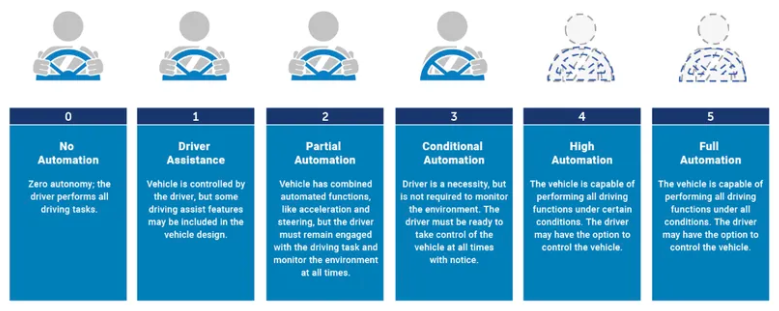
\includegraphics[width=12cm]{figs/introducción/niveles.png}
  \end{center}
  \caption{Niveles de autonomía explicados(\ac{SAE}).}
  \label{aut-levels}
  \end{figure}

\begin{itemize}
    \item \textit{Nivel 0:} Ninguna autonomía. El conductor es completamente responsable de todas las tareas de conducción.
    \item \textit{Nivel 1:} Asistencia al conductor. El vehículo puede realizar una función específica (como el control de crucero), pero siempre requiere la supervisión activa del conductor.
    \item \textit{Nivel 2:} Automatización parcial. El vehículo cuenta con sistemas que pueden replicar tareas del conductor, pero el conductor debe estar preparado para intervenir en cualquier momento.
    \item \textit{Nivel 3:} Automatización condicional. El vehículo puede tomar control completo en determinadas condiciones, pero el conductor debe estar disponible para retomar el control si el sistema lo solicita. Un ejemplo destacado de este nivel es el Autopilot de Tesla.
    \item \textit{Nivel 4:} Alta automatización. El vehículo puede operar de forma autónoma en condiciones específicas, sin necesidad de intervención humana, aunque pueden existir limitaciones geográficas o contextuales.
    \item \textit{Nivel 5:} Automatización total. El vehículo es completamente autónomo y no requiere intervención humana en ningún momento ni bajo ninguna circunstancia.
\end{itemize}

Hoy en día, no existen vehículos completamente autónomos disponibles comercialmente. Lo más cercano a la autonomía total que se puede encontrar en el mercado es el nivel 2+. Sin embargo, existen numerosos proyectos en desarrollo que están alcanzando el nivel 3, como es posible ver videos promocionales que muestran coches en movimiento sin intervención activa del conductor. No obstante, estas demostraciones se realizan en entornos extremadamente controlados y con condiciones específicas.

En algunos países, la legislación aún no permite el uso de vehículos autónomos de nivel 3 o superior. Por ejemplo, en España, la ley prohíbe que el conductor suelte el volante durante la conducción, lo que impide el uso de vehículos de nivel 3. En cambio, en California, es legal el uso de vehículos con conducción semi-autónoma, lo que permite al conductor levantar las manos del volante en ciertas circunstancias \cite{carwow-autonomous}.

\subsection{Evolución histórica de los vehículos autónomos}
\label{sec:historia}

La primera vez que se puso en práctica el concepto de vehículo autónomo fue en 1925 en Nueva York. El ingeniero Francis Houdina diseñó el primer coche sin conductor, controlado de forma remota por radiofrecuencia. Sin embargo, este vehículo requería un coche escolta desde el cual se dirigía.

En 1939, el diseñador industrial estadounidense Norman Bel Geddes revolucionó las ideas sobre transporte al presentar, en la Feria Futurama, un concepto visionario: vehículos eléctricos guiados de manera autónoma mediante radiocontrol en carreteras automáticas con circuitos eléctricos integrados en el pavimento. Aunque no se trataba del concepto moderna de coche autónomo, esta propuesta marcó un antes y un después, despertando el interés de numerosas empresas tecnológicas en el campo de la conducción autónoma.

\begin{figure} [ht]
  \begin{center}
    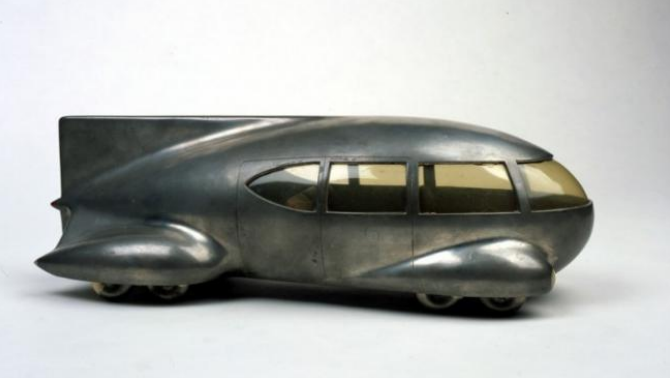
\includegraphics[width=12cm]{figs/introducción/coche_geddes.png}
  \end{center}
  \caption{Coche diseñado por Norman Bel Geddes en 1933.}
  \label{coche-geddes}
  \end{figure}

La mayoría de los avances significativos en este ámbito se deben a Ernst Dickmanns, un profesor alemán experto en \ac{IA}. Dickmanns lideró la creación del primer coche autónomo moderno, combinado la visión sacádica (un movimiento
rápido del ojo, cabeza u otras partes del cuerpo de animales o dispositivos) con cálculos probabilísticos y computación paralela. En 1987, diseñó una furgoneta \textit{Mercedes-Benz} equipada con esta tecnología, logrando conducirla exitosamente por una autopista a velocidades de hasta 100 km/h en condiciones de tráfico controladas. En 1994, lo superó con el modelo  \textit{Mercedes 500 SEL}, conocido como \textit{VaMP}, que recorrió más de 1.000 kilómetros en la carretera de circunvalación de París. Este vehículo alcanzó velocidades de hasta 130 km/h y era capaz de realizar maniobras complejas, como adelantamientos.

\begin{figure}[ht]
  \begin{center}
    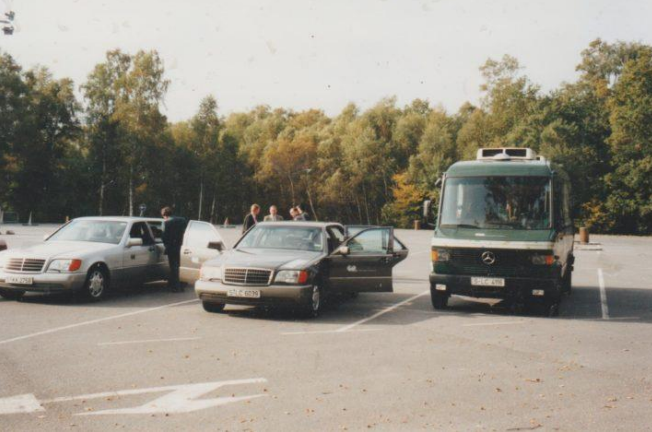
\includegraphics[width=8cm]{figs/introducción/paris_1994.png}
  \end{center}
  \caption{Demostración en vico del funcionamiento de \textit{VaMP} en París.}
  \label{coche-geddes}
\end{figure}

La Comisión Europea, consciente del potencial de los coches autónomos, destinó 800 millones de euros al proyecto  \textit{EUREKA Prometheus}, una iniciativa que marcó un hito en el desarrollo de esta tecnología. Este programa facilitó la creación de numerosos prototipos que sentaron las bases de los vehículos autónomos modernos  \cite{history-vehicles}. Actualmente, este campo es liderado por empresas como  \textit{Waymo},  \textit{Tesla},  \textit{Cruise} y  \textit{NVIDIA } \cite{ai-self-driving-cars}.

\textit{Waymo} \footnote{\url{https://waymo.com/intl/es/}}, el sistema de conducción autónoma desarrollado por \textit{Google}, se ha consolidado como un referente en el sector de los vehículos sin conductor. Gracias a la integración de \ac{IA}, \textit{Waymo} destaca por su capacidad para planificar rutas complejas y reaccionar de forma inteligente ante diversos escenarios en la carretera. Un vehículo \textit{Waymo} es capaz de operar de manera segura y autónoma siguiendo los siguientes pasos:

\begin{itemize}
    \item El conductor o pasajero establece el destino y el software del vehículo calcula automáticamente la mejor ruta.
    \item Un sensor \textit{LIDAR} giratorio, montado en el techo, escanea un rango de 60 metros alrededor del vehículo, generando un mapa tridimensional dinámico del entorno.
    \item Un sensor ubicado en la rueda trasera izquierda mide los movimientos laterales del vehículo para determinar su posición exacta en relación con el mapa 3D.
    \item Los sistemas de radar, instalados en los parachoques delantero y trasero, calculan la distancia a los obstáculos cercanos.
    \item La inteligencia artificial del vehículo recopila datos de todos los sensores, así como de \textit{Google Street View} y cámaras internas, para interpretar el entorno y tomar decisiones.
    \item La \ac{IA} simula los procesos perceptivos y de toma de decisiones de un ser humano mediante aprendizaje profundo, controlando sistemas clave como los frenos y la dirección.
    \item El software del vehículo consulta \textit{Google Maps} para obtener información anticipada sobre señales de tráfico, puntos de referencia y semáforos.
\end{itemize}

\begin{figure}[ht]
  \begin{center}
    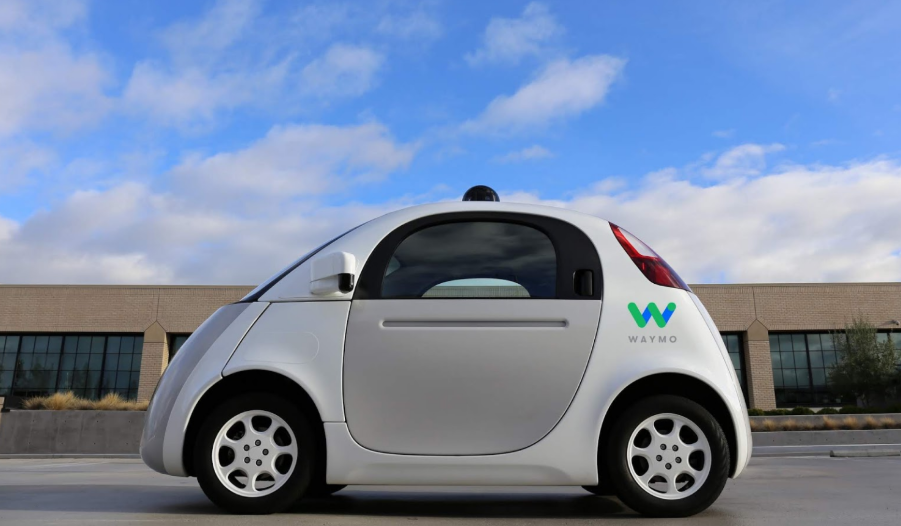
\includegraphics[width=7cm]{figs/introducción/waymo.png}
  \end{center}
  \caption{Coche autónomo de Waymo con sensores y tecnología avanzada.}
  \label{waymo}
\end{figure}

Tesla ha logrado un avance notable con su sistema \textit{Autopilot}, capaz de mantener un control preciso utilizando sofisticados algoritmos de inteligencia artificial para tomar decisiones rápidas y precisas. Modelos como el \textit{Model 3} y el \textit{Model Y} han implementado el sistema \textit{Tesla Vision}, que prescinde del uso de radar y utiliza un avanzado conjunto de cámaras junto con el procesamiento de redes neuronales desarrolladas por Tesla. Este sistema ofrece tres niveles principales: Piloto automático, Piloto automático mejorado y Capacidad de conducción autónoma total.

\begin{itemize}
    \item \textbf{Piloto Automático}
    \begin{itemize}
        \item \textit{Control de crucero adaptativo al tráfico}: ajusta automáticamente la velocidad del vehículo para adecuarse al flujo del tráfico.
        \item \textit{Autogiro}: permite mantener al vehículo dentro de un carril claramente delimitado.
    \end{itemize}
    \item \textbf{Piloto Automático Mejorado}
    \begin{itemize}
        \item \textit{Cambio automático de carril}: facilita el cambio al carril adyacente cuando el conductor activa el intermitente.
        \item \textit{Navegar en piloto automático (Beta)}: mejora la funcionalidad de cambio de carril automático al proporcionar orientación activa para transitar desde la incorporación hasta la salida de autovías. Incluye sugerencias de cambio de carril y asistencia en intersecciones.
        \item \textit{Autopark}: automatiza el proceso de estacionamiento en paralelo o perpendicular.
        \item \textit{Dumb Summon}: permite mover el vehículo dentro o fuera de plazas de aparcamiento estrechas mediante la aplicación móvil.
        \item \textit{Actually Smart Summon}: mejora las capacidades del vehículo para moverse de manera autónoma en entornos complejos, como plazas de aparcamiento, maniobrando alrededor de obstáculos y localizando al conductor dentro del área cercana.
    \end{itemize}
    \item \textbf{Capacidad de Conducción Autónoma Total}
    \begin{itemize}
        \item \textit{Integración completa}: incluye todas las funcionalidades del Piloto Automático básico y del Piloto Automático Mejorado.
        \item \textit{Control de semáforos y señales de stop (Beta)}: detecta señales de tráfico como semáforos y señales de alto. A medida que el vehículo se acerca, ajusta automáticamente la velocidad y se detiene.
    \end{itemize}
\end{itemize}

A pesar de las mejoras en el rendimiento que proporcionan estas características, no hacen que el coche sea autónomo, requieren un conductor totalmente atento, con las manos en el volante y preparado para tomar el control en cualquier momento \cite{tesla-autopilot}.

\begin{figure}[ht]
  \begin{center}
    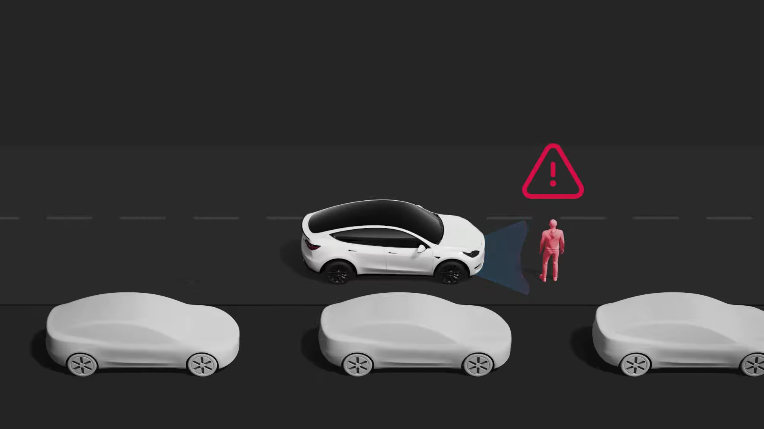
\includegraphics[width=9cm]{figs/introducción/tesla_model_y.png}
  \end{center}
  \caption{\textit{Tesla Model Y} frenando ante un obstáculo.}
  \label{tesla}
\end{figure}

\textit{Cruise}, una empresa de \textit{General Motors}, ha destacado con su vehículo \textit{Cruise AV}, en el que el 40\% de su hardware está diseñado específicamente para la conducción autónoma. Este modelo integra una combinación de cámaras, \textit{LIDAR} y radar, permitiéndole realizar entre 200 y 800 maniobras diarias para sortear vehículos estacionados en doble fila \footnote{\url{https://www.getcruise.com/news/blog/2019/how-self-driving-cars-think-navigating-double-parked-vehicles/?_gl=1*81u4mi*_gcl_au*MTU2MzE4NjQzOC4xNzM2Njg4NzY2s}}. Además, el sistema es capaz de adaptarse a condiciones climáticas adversas, como la lluvia, asegurando una conducción segura y eficiente en entornos urbanos complejos.

\begin{figure}[ht]
  \begin{center}
    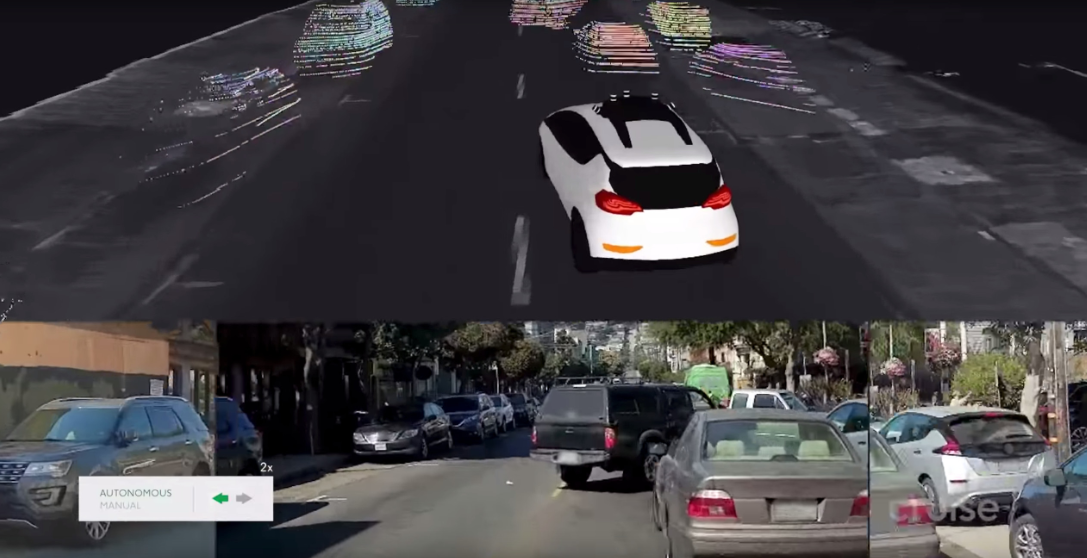
\includegraphics[width=9cm]{figs/introducción/cruise_av.png}
  \end{center}
  \caption{Detección de otros coches del \textit{Cruise AV}.}
  \label{cruise}
\end{figure}

Por último, \textit{NVIDIA} ha desarrollado la plataforma \textit{NVIDIA DRIVE} \footnote{\url{https://www.nvidia.com/es-es/self-driving-cars/?utm_source}}, una solución de computación avanzada que demuestra cómo la inteligencia artificial puede integrarse de manera efectiva en los vehículos autónomos.

\begin{figure}[ht]
  \begin{center}
    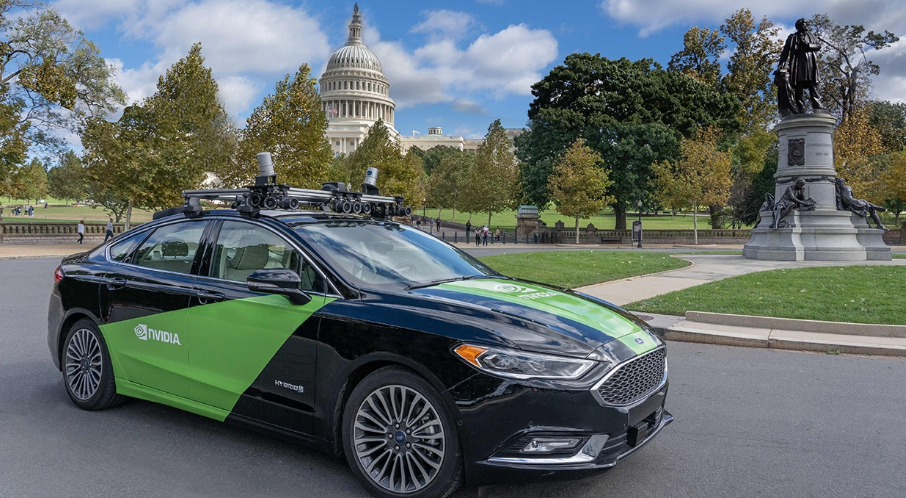
\includegraphics[width=7cm]{figs/introducción/nvidia.png}
  \end{center}
  \caption{Coche autónomo de NVIDIA.}
  \label{nvidia}
\end{figure}

\subsection{Desafíos actuales en la implementación de vehículos autónomos}
\label{sec:desafíos}

Los vehículos autónomos enfrentan numerosos desafíos que deben ser superados para lograr su implementación generalizada. Estos desafíos se dividen principalmente en aspectos técnicos y no técnicos, cada uno con sus propias complejidades que requieren soluciones específicas.

En el ámbito técnico, uno de los mayores retos radica en la detección y análisis de datos. Los vehículos autónomos necesitan identificar obstáculos de manera inequívoca, incluso a altas velocidades y largas distancias. Esto exige un software avanzado capaz de procesar grandes volúmenes de datos en tiempo real con un alto grado de precisión, un área que aún enfrenta importantes limitaciones. Además, garantizar un sistema seguro y fiable implica desarrollar tecnología tolerante a fallos y capaz de operar de manera eficiente en entornos no controlados. En el mundo real, los vehículos autónomos deben enfrentarse a miles de situaciones impredecibles durante la conducción, y los sistemas actuales todavía están lejos de resolver de manera eficiente todas estas incertidumbres.

Otro desafío técnico crucial es la seguridad cibernética. Los vehículos autónomos, especialmente aquellos basados en \ac{DL}, son vulnerables a ataques que podrían comprometer su funcionalidad o la seguridad de sus ocupantes. Por ello, es imprescindible implementar estrategias robustas de defensa para mitigar estos riesgos y generar confianza en la tecnología.

En el ámbito no técnico, las cuestiones legales y éticas presentan una barrera importante. Existe una preocupación creciente sobre la responsabilidad en caso de accidentes, ya que no está claro si la culpa recaería en el fabricante, el desarrollador del software o el propietario del vehículo. También es esencial salvaguardar la privacidad de los datos de los pasajeros, ya que los sistemas autónomos recopilan y procesan grandes cantidades de información personal.

La aceptación por parte de los consumidores y las regulaciones gubernamentales son factores determinantes en el desarrollo de vehículos autónomos. En la actualidad, las políticas y normativas suelen avanzar a un ritmo más lento que el desarrollo tecnológico, lo que complica las pruebas y la implementación a gran escala.

La superación de estos obstáculos requerirá soluciones innovadoras que satisfagan las necesidades de los consumidores, la industria y los gobiernos. La colaboración interdisciplinaria será clave para abordar estos desafíos, sentando las bases de un futuro en el que los vehículos autónomos sean seguros, eficientes y ampliamente aceptados en la sociedad \cite{challenges-autonomous}.

\section{Impacto de la IA en el transporte autónomo}
\label{sec:ia-intro}

\chapter{Objetivos}
\label{cap:capitulo2}

En esta sección del documento se describe el problema a resolver, marcando los objetivos y requisitos pautados en el desarrollo del \ac{TFG}.

\section{Descripción del problema}
\label{sec:descripcion}

El objetivo principal de este \ac{TFG} es desarrollar un primer paso para un sistema de conducción autónoma capaz de desenvolverse eficientemente en entornos urbanos. Para lograrlo, se emplean técnicas de \ac{DRL} para la toma de decisiones, junto con diferentes enfoques de \ac{DL} para la percepción del entorno, con el objetivo de garantizar un comportamiento robusto, seguro y eficiente. El proyecto se centra en conseguir una conducción segura y estable durante todo el recorrido, abordando tres tareas principales: seguimiento del carril, control de crucero adaptivo y llevar a cabo una maniobra de adelantamiento completa.

A continuación, se definen los siguientes sub-objetivos: 

\begin{enumerate}
\item Implementación de un módulo de percepción basado en el \ac{LiDAR} para identificar obstáculos en la carretera y en cámaras RGB, combinadas con técnicas de \ac{DL} para el post-procesado, para la segmentación de la calzada y detección del carril.
\item Desarrollo de un comportamiento de sigue-carril.
\item Ampliación del comportamiento de seguimiento de carril para incorporar una respuesta adaptativa al tráfico, manteniendo una velocidad de crucero ajustada al vehículo que circula delante del coche autónomo.
\item Desarrollo de un modelo capaz de ejecutar maniobras completas de adelantamiento, incluyendo el cambio de carril y la vuelta al mismo.
\item Análisis y comparación de los diferentes comportamientos de conducción autónomos desarrollados.
\end{enumerate}

\section{Requisitos}
\label{sec:requisitos}

Los requisitos que han de cumplirse en este trabajo son:
\begin{enumerate}
\item Uso del entorno de simulación CARLA\footnote{\url{https://carla.org/}}, el cual permite la simulación de escenarios realistas, diversos comportamientos de vehículos y la prueba de modelos. Al ser un simulador ampliamente reconocido en el ámbito de la conducción autónoma, garantiza la reutilización del proyecto en aplicaciones futuras de este campo.
\item Usar modelos de \ac{DL} para la percepción visual y algoritmos de \ac{DRL} para la toma de decisiones.
\item Lograr un comportamiento sigue-carril estable y sin oscilaciones, alcanzando velocidades en torno a los 70 km/h.
\item Mantener un control de crucero adaptativo respecto al vehículo delantero, asegurando una distancia de seguridad adecuada respecto al vehículo delantero, de acuerdo con las normas de la \ac{DGT}\footnote{\url{https://www.dgt.es/export/sites/web-DGT/.galleries/downloads/conoce-el-estado-del-trafico/operaciones-especiales/4_O.-E.-Primero-de-Mayo-2023_Consejos-y-normas-de-Seguridad-Vial_V-I.pdf}}.
\item Llevar a cabo un adelantamiento seguro en todo momento, comprobando si existe un carril al que podamos desplazarnos y asegurando que la maniobra de retorno al carril inicial no pone en peligro al otro agente en la vía.
\end{enumerate}

\section{Metodología}
\label{sec:metodologia}

Este TFG comenzó en febrero de 2024 y finalizó en marzo de 2025. La metodología de trabajo fue la siguiente:

\begin{itemize}
\item Se ha utilizado la metodología \textit{Scrum}\footnote{\url{https://www.nimblework.com/agile/scrum-methodology/}}, la cual consiste en organizar el trabajo en ciclos cortos llamados \textit{sprints}, que suelen durar entre una y cuatro semanas. Esta metodología fomenta una organización eficiente al dividir el trabajo en tareas pequeñas y manejables, promoviendo la iteración y mejora continua al revisar y ajustar el trabajo regularmente.
\item Durante cada \textit{sprint}, se realizaron reuniones semanales a través de \textit{Teams}\footnote{\url{https://www.microsoft.com/es-es/microsoft-teams/log-in}}, con una duración de 30-60 minutos, para hacer un seguimiento de los problemas que hubieran podido surgir a lo largo de la semana y definir los nuevos objetivos a cumplir.
\item Contacto mediante el email de la universidad con el fin de resolver problemas urgentes e intercambiar contenido de avances significativos.
\item Se utilizó un repositorio de \textit{GitHub}\footnote{\url{https://github.com/RoboticsLabURJC/2024-tfg-lara-poves/}} para gestionar el control de versiones del código fuente, los modelos y los datos más relevantes generados durante el desarrollo del proyecto. En la Figura \ref{fig:github}, se observa que la mayor carga de trabajo tuvo lugar al inicio, coincidiendo con la creación de los entornos de desarrollo y la implementación del módulo de percepción. Posteriormente, se llevaron a cabo los entrenamientos y pruebas de los modelos, ajustando los hiperparámetros de entrenamiento e intentando mejorar los resultados obtenidos. Finalmente, se ve un último \textit{sprint} referente a la elaboración de la memoria y a los ajustes finales en los entrenamientos del adelantamiento.

\begin{figure}[ht]
\centering
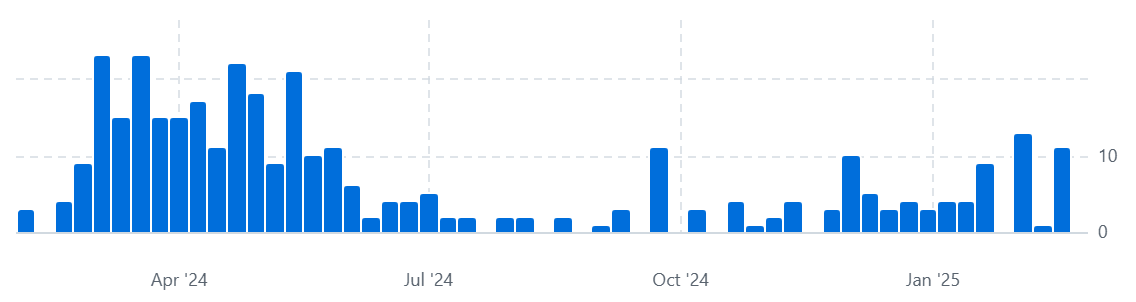
\includegraphics[width=9cm]{figs/objetivos/github.png}
\caption{Seguimiento de trabajo en GitHub.}
\label{fig:github}
\end{figure}

\item Mantenimiento de un \textit{blog}\footnote{\url{https://roboticslaburjc.github.io/2024-tfg-lara-poves/}} con el propósito de documentar problemas, avances e investigaciones realizadas durante el desarrollo del proyecto, asegurando un registro del progreso y soluciones a los desafíos plateados.

\end{itemize}

\section{Plan de trabajo}
\label{sec:plantrabajo}

Finalmente, los pasos a seguir fueron:

\begin{enumerate}
\item Comienzo del trabajo:
\begin{itemize}
\item Desde el inicio, el tema del proyecto estuvo claro, centrado en la conducción autónoma en el simulador CARLA y algoritmos de \ac{DRL}.
\item Se gestionó el acceso al servidor donde se desarrollaría el proyecto, el cual ya contaba con el simulador CARLA instalado. 
\item Se creó un entorno \textit{Anaconda} y se procedió a la instalación de las librerías necesarias para el desarrollo del proyecto.
\end{itemize}

\item Desarrollo del proyecto:
\begin{itemize}
\item Se desarrolló un teleoperador sencillo para explorar las diversas funcionalidades y configuraciones que ofrece el simulador CARLA.
\item Se implementó el manejo y visualización de los sensores, \ac{LiDAR} y cámara RGB, cuyos datos se utilizarán posteriormente para lograr los comportamientos autónomos. Además, se integraron redes neuronales para la detección del carril y la segmentación semántica de la calzada. También se incluyó una nueva forma de detección del carril basada en \textit{ground truth} en CARLA. 
\item A partir de los datos de los sensores y las herramientas integradas, se implementó la detección del carril, calculando variables como su área y centro de masas. Además, se aplicó un tratamiento inteligente a la nube de puntos del \ac{LiDAR}, filtrando estos puntos para detectar otros vehículos en la carretera.
\item Se configuró el autopiloto de CARLA explorando sus opciones disponibles.
\item Se desarrolló un sistema sigue-carril basado en un controlador \ac{PID}.
\item En una primera etapa, se entrenó un modelo utilizando el algoritmo \ac{DQN} para el seguimiento de carril, pero posteriormente, se entrenó un nuevo modelo basado en \ac{PPO} para mejorar el desempeño.
\item Se reentrenó el modelo basado en \ac{PPO} para lograr un control de crucero adaptativo utilizando la información proporcionada por el \ac{LiDAR}.
\item Finalmente, se entrenó un nuevo modelo para conseguir realizar una maniobra de adelantamiento completa.
\end{itemize}

\item Evaluación: Se compararon y analizaron los resultados obtenidos durante las diferentes fases y modelos del proyecto.
\item Se redactó la memoria del trabajo, documentando todo el proceso de investigación y desarrollo realizado.
\end{enumerate}


\chapter{Plataformas de desarrollo}
\label{cap:capitulo3}

En este capítulo se describen en detalle las tecnologías y herramientas empleadas durante el desarrollo de este \ac{TFG}, incluyendo el simulador, las herramientas de percepción, el editor, así como el lenguaje de programación y las librerías utilizadas. Además, se expone el hardware empleado para llevar a cabo los entrenamientos.

\section{Lenguajes de programación}
\label{sec:programación}
\subsection{Python}
\label{sec:python}

Python\footnote{\url{https://www.python.org/}} es un lenguaje de programación de alto nivel\footnote{\url{https://www.tecnologia-informatica.com/lenguaje-de-alto-nivel-que-es-ejemplos/}} interpretado\footnote{\textbf{Lenguaje de programación interpretado}: Lenguaje en el que las implementaciones se ejecutan directamente, sin necesidad de compilar el programa ni generar código máquina del mismo.} que ha ganado gran popularidad en los últimos años gracias a su simplicidad, versatilidad y enfoque multiparadigma\footnote{\textbf{Multiparadigma:} soporta programación orientada a objetos, funcional y procedimental.}. Posee una extensa colección de librerías que facilitan el desarrollo de aplicaciones en áreas muy diversas.

En este \ac{TFG}, Python 3 se emplea para el desarrollo completo del código, utilizando diversas bibliotecas tanto para la creación de entornos de entrenamiento y prueba de modelos, como para la implementación de comportamientos basados en \ac{DRL}.

\subsubsection{Pygame}
\label{sec:pygame}

Pygame\footnote{\url{https://www.pygame.org/docs/}} es una librería de Python ampliamente utilizada para el desarrollo de juegos y aplicaciones multimedia. Proporciona un conjunto de herramientas que permite crear gráficos, visualizar imágenes y gestionar animaciones de manera sencilla y eficiente. Además, Pygame ofrece funcionalidades para la captura y el manejo de eventos de entrada, como las pulsaciones de teclas y los clics del ratón.

\begin{code}[h]
\begin{lstlisting}[language=Python]
import pygame

# Setup
pygame.init()
screen = pygame.display.set_mode(size, pygame.HWSURFACE | pygame.DOUBLEBUF)
pygame.display.set_caption(name)

while True:
	for event in pygame.event.get():
		if event.type == pygame.QUIT:
			pygame.quit()
			break

	screen.fill("purple") # Fill the screen with a color
	pygame.display.flip() # Display your work on the screen
\end{lstlisting}
\caption[Ejemplo de código en Python utilizando Pygame]{Ejemplo de código en Python utilizando Pygame para mostrar una interfaz gráfica}
\label{cod:pygame}
\end{code}

En este caso, se ha utilizado Pygame para desarrollar la interfaz gráfica del proyecto, permitiéndonos visualizar la nube de puntos del \ac{LiDAR} y las imágenes de las cámaras, incluyendo la detección del carril y clasificación de objetos.

\begin{figure}[ht]
\begin{center}
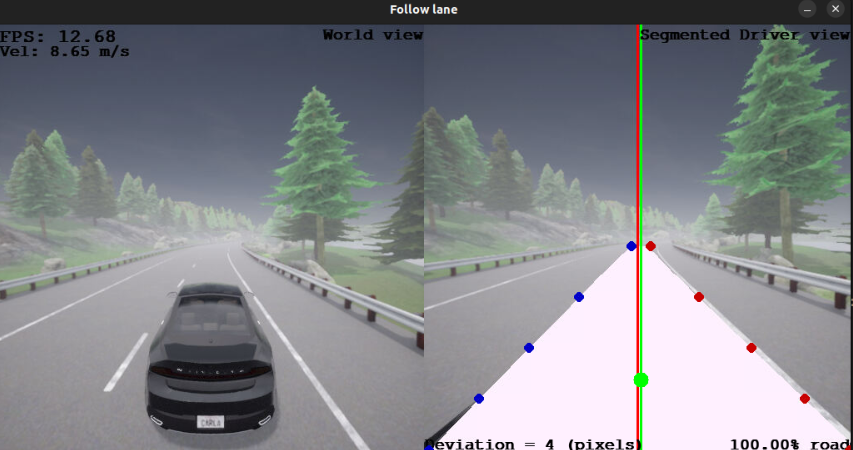
\includegraphics[width=12cm]{figs/Plataformas_Desarollo/pygame.png}
\end{center}
\caption{Interfaz gráfica desarrollada con Pygame donde se visualiza la detección del carril y el \ac{LiDAR}.}
\label{foto_pygame}
\end{figure}

\subsubsection{NumPy}
\label{sec:numpy}

NumPy\footnote{\url{https://numpy.org/}} es una librería de Python que proporciona soporte para matrices y ofrece una extensa colección de funciones matemáticas y operaciones optimizadas para trabajar con estos arreglos. Es ampliamente utilizada por su eficiencia computacional y facilidad de uso. En este proyecto, ha sido muy útil para manejar los \textit{arrays} utilizados para clasificar los puntos del \ac{LiDAR}y las matrices de imágenes y máscaras, permitiéndonos analizar y filtrar estos datos de manera eficiente.

\begin{code}[h]
\begin{lstlisting}[language=Python]
import numpy as np

index = np.argwhere(self._mask == ROAD)
index_sorted = index[np.argsort(index[:, 0])] # Sorted by y

\end{lstlisting}
\caption[Ejemplo de indexación y ordenación de datos con NumPy]{Ejemplo de indexación y ordenación de datos con NumPy}
\label{cod:numpy}
\end{code}

\subsubsection{Matplotlib}
\label{sec:plot}

La librería Matplotlib\footnote{\url{https://matplotlib.org/}} es una herramienta muy popular en Python para crear gráficos y otras visualizaciones. Permite generar todo tipo de diagramas, como líneas, barras o histogramas. Es comúnmente utilizada gracias a su flexibilidad para personalizar los gráficos y su integración con otras librerías como NumPy y Pandas\footnote{\url{https://pandas.pydata.org/}}, librería de Python para la manipulación y análisis de datos. Además, ofrece la posibilidad de exportar los gráficos en diversos formatos. En este \ac{TFG}, se ha utilizado principalmente para la visualización de los datos recopilados durante la inferencia y a lo largo de los entrenamientos.

\begin{code}[h]
\begin{lstlisting}[language=Python]
import matplotlib.pyplot as plt
import matplotlib.patches as mpatches

if points:
	# Scatter plot with colors based on finish
	color_map = {0: 'red', 1: 'green'}
	plt.scatter(range(len(data)), data, color=[color_map[f] for f in finish], s=7)
	
	# Legend
	red_patch = mpatches.Patch(color='red', label='Finish = False')
	green_patch = mpatches.Patch(color='green', label='Finish = True')
	plt.legend(handles=[red_patch, green_patch])  
else:
	plt.plot(range(len(data)), data, linewidth=1, label=key)
	cumulative_avg = np.cumsum(data) / np.arange(1, len(data) + 1)
	plt.plot(range(len(data)), cumulative_avg, label=label, linewidth=2.5)
	plt.legend()

plt.ylabel(key)
plt.xlabel('Episode')
plt.title(title)
\end{lstlisting}
\caption[Ejemplo de código en Python para visualizar datos con Matplotlib]{Ejemplo de código en Python para visualizar datos con Matplotlib.}
\label{cod:plot}
\end{code}

\begin{figure}[ht]
  \begin{center}
    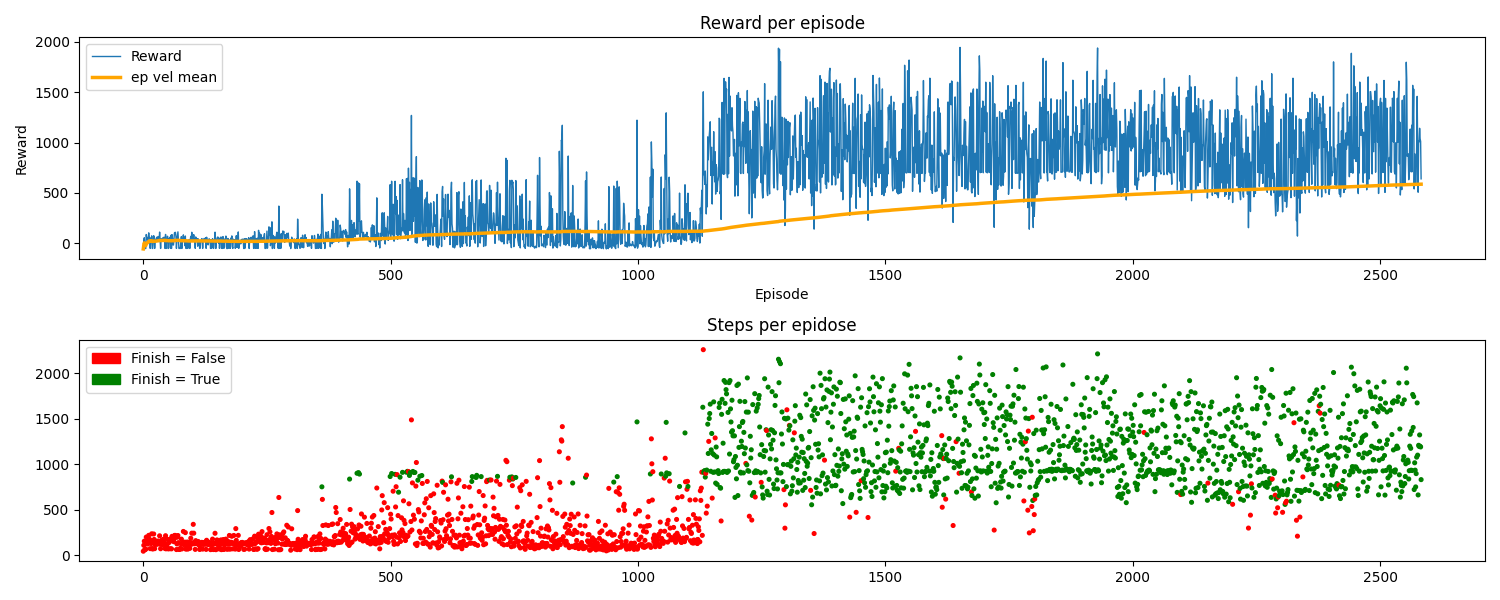
\includegraphics[width=12cm]{figs/Plataformas_Desarollo/plot.png}
  \end{center}
  \caption{Ejemplo de gráficas de datos de entrenamiento con Matplotlib.}
  \label{foto_plot}
\end{figure}

\subsubsection{Gymnasium}
\label{sec:gymnasium}

Gymnasium\footnote{\url{https://pypi.org/project/gymnasium/}} es una biblioteca de Python desarrollada por OpenAI\footnote{\url{https://openai.com//}}, que proporciona herramientas para crear una amplia variedad de entornos, diseñados específicamente para aplicar y probar algoritmos de aprendizaje por refuerzo.

En nuestro proyecto de conducción autónoma, hemos utilizado la biblioteca Gymnasium, combinada con el simulador CARLA, para crear los entornos de entrenamiento y prueba de nuestros modelos. Para ello, es necesario definir una clase personalizada que herede de la clase base \textit{Env} proporcionada por Gymnasium. En esta clase, configuramos las variables necesarias, como el espacio de observaciones, e implementamos los métodos fundamentales para el entrenamiento, \textit{step}, \textit{reset} y \textit{close}. En la fragmento de código \ref{cod:gym}, se muestra un ejemplo básico de implementación en Python.

Los métodos \textit{step} y \textit{reset} son fundamentales para ejecutar un algoritmo de aprendizaje por refuerzo, ya que permiten la interacción entre el agente y el entorno. La función \textit{step} recibe como entrada la acción tomada por el agente y devuelve una tupla con las nuevas observaciones del entorno, la recompensa obtenida, indicadores de si el episodio ha terminado, si ha sido truncado y un diccionario con información adicional. Por otro lado, la función \textit{reset} se utiliza al comienzo de cada episodio para reiniciar el entorno y otras variables a su estado inicial, devolviendo la primera observación y su información asociada. Juntos, estos métodos estructuran el ciclo iterativo de simulación y aprendizaje, asegurando consistencia en el entrenamiento y permitiendo al agente adquirir conocimeintos y mejorar su desempeño a lo largo de múltiples episodios.

\begin{code}[H]
\begin{lstlisting}[language=Python]

import gymnasium as gym

class CarlaBase(gym.Env):
    def __init__(self):
        self.observation_space = obs_space
    
    def _get_obs(self):
        return obs
    
    def _get_info(self):
        return info
    
    def step(self, action: np.ndarray):
        return self._get_obs(), reward, terminated, truncated, self._get_info()
   
    def reset(self, seed=None):
        return self._get_obs(), self._get_info()
    
    def close(self):
        # Destroy CARLA actors
        pygame.quit()

\end{lstlisting}
\caption[Definición de un entorno personalizado en Gymnasium]{Definición de un entorno personalizado con Gymnasium.}
\label{cod:gym}
\end{code}

El espacio de observaciones es una descripción formal que define el tipo, la estructura y los límites de los datos que el agente puede recibir del entorno en cada momento. Funciona como un marco que delimita la información accesible para el agente. En Gymnasium, este espacio se configura mediante clases predefinidas, como \textit{Box}, \textit{Discrete} o \textit{Dict}, estableciendo el rango permitido y la estructura de los datos. Esta configuración debe ser compatible con la política del modelo de aprendizaje utilizado, ya que define la entrada que la red neuronal o algoritmo de decisión del agente. En nuestro caso, como utilizaremos una política basada en diccionarios, crearemos el espacio de observaciones continuo mediante la clase \textit{Dict}, la cual permite combinar múltiples espacios de observación en una estructura organizada.

\begin{code}[H]
\begin{lstlisting}[language=Python]

self.observation_space = spaces.Dict(
	spaces={
		KEY_CM: spaces.Box(
			low=0,
			high=SIZE_CAMERA - 1,
			shape=(2,),
			dtype=np.int32
		),
		KEY_LEFT_POINTS: spaces.Box(
			low=0,
			high=SIZE_CAMERA - 1,
			shape=(self._num_points_lane, 2),
			dtype=np.int32
		)
	}
)

\end{lstlisting}
\caption[Definición del espacio de observaciones en un entorno Gymnasium]{Definición del espacio de observaciones en un entorno Gymnasium.}
\label{cod:gymobs}
\end{code}

\subsubsection{Stable-Baselines3}
\label{sec:stable_baselines3}

Stable-Baselines3\footnote{\url{https://stable-baselines3.readthedocs.io/en/master/}} es una librería de Python que proporciona implementaciones estables y fáciles de usar de algoritmos de aprendizaje por refuerzo basadas PyTorch\footnote{\url{https://pytorch.org/}} como \textit{backend}. Además, incluye compatibilidad con TensorBoard\footnote{\url{https://www.tensorflow.org/tensorboard?hl=es-419}}, lo que permite visualizar métricas del entrenamiento en tiempo real y analizar el rendimiento de los modelos. 

De esta librería, utilizaremos algunos algoritmos basados en \ac{DRL} es un enfoque en el que los agentes de aprendizaje por refuerzo utilizan redes neuronales para tomar decisiones. Esta combinación les permite adaptarse mejor a entornos complejos donde las reglas no son evidentes ni fácilmente definibles, como es el caso de la conducción autónoma. Dentro de los algoritmos de \ac{DRL}, existen dos tipos claramente diferenciados:

\begin{itemize}
\item \textit{On-policy:} Son aquellos que actualizan el modelo solo con datos de la política actual, una vez que la política cambia, los datos anteriores se vuelven inservibles y se descartan.
\item \textit{Off-policy:} Son aquellos que pueden usar cualquier dato recolectado durante el entrenamiento, independientemente de la política con la que hayan sido obtenidos.
\end{itemize}

En concreto, en este \ac{TFG} utilizaremos los algoritmos de \ac{DQN} y \ac{PPO}. \ac{DQN} es un algoritmo de \ac{DRL} que soportar un espacio de estados complejo y continuo, pero el espacio de acciones es discreto. Las acciones en un espacio discreto son predefinidas y limitadas, es decir, no existe una continuidad entre ellas, sino que están representadas por un número finito de opciones que el agente puede elegir en cada estado.

\ac{DQN} es un algoritmo \textit{off-policy} ya que incluye una \textit{replay memory}. Esta técnica consiste en crear una memoria de reproducción de experiencias que almacena las k experiencias más recientes que un agente ha recopilado, ya que son las más relevantes, para así poder reutilizarlas. Si la memoria está llena, se descarta la experiencia más antigua para dar espacio a la más reciente. En cada paso de entrenamiento, se muestrea uno o más lotes de datos de forma aleatoria de la memoria para actualizar los parámetros de la red. El tamaño de la memoria debe ser lo suficientemente grande como para contener experiencias de diferentes episodios y políticas, lo que ayuda estabilizar y mejorar el entrenamiento. Al actualizar en cada paso del entrenamiento la red neuronal, la minimización del error entre las predicciones de la red y los valores reales se vuelve complicada. Para abordar este problema, se introduce una nueva red neural, \textit{target network}, diseñada para aportar estabilidad al proceso de entrenamiento. La nueva red es una réplica de la red principal, \textit{policy network}, pero en lugar de actualizarla en cada paso, la igualamos a la red original cada cierto número de pasos, manteniendo un objetivo de entrenamiento constante \cite{drl}.

El algoritmo \textit{Actor-Critic} es un tipo de algortimo en el que cada agente consta de dos elementos que aprenden de manera conjunta, cada uno con su propia red neuronal: \textit{actor}, encargado de aprender la política óptima, y \textit{critic}, responsable de aprender la función de valor y proporcionar una señal de refuerzo a la política. El algoritmo \ac{A2C} se forma a partir de la unión del actor y el critic y es una algoritmo \textit{on-policy}. \ac{PPO} es un algoritmo \textit{on-policy} que puede considerarse como una extensión de \ac{A2C}, cuyo objetivo principal es evitar el deterioro del rendimiento. En los algoritmos basados en políticas, ajustar la tasa de aprendizaje puede ser una labor complicada. Un valor pequeño puede llevar a entrenamientos prolongados sin alcanzar la solución óptima, mientras que uno grande puede causar un colapso en el rendimiento. Con el objetivo de resolver esto, \ac{PPO} introduce un objetivo sustituto que asegura una mejora monótona del rendimiento, evitando cambios drásticos y arriesgados en la política que puedan afectar negativamente al despeño. Para lograrlo, \ac{PPO} mide cuánto ha cambiado la política después de cada actualización, garantizando que esta diferencia sea no negativa en cada iteración, asegurando así una mejora continua en el rendimiento. Además, que impide que esta razón crezca o disminuya demasiado dentro de un umbral controlado por un hiperparámetro (\textit{clip\_range}) \cite{drl}. 

Dependiendo del escenario, puede ser necesario utilizar diferentes estructuras de datos para proporcionar las observaciones al modelo. Stable-Baselines3 ofrece tres tipos de políticas que permiten adaptar el modelo a distintas formas de entrega de los datos:

\begin{itemize} 
\item \textit{MlpPolicy:} Diseñada para trabajar con estados en forma de vectores, como en el entorno \textit{CartPole}\footnote{\url{https://gymnasium.farama.org/environments/classic_control/cart_pole/}}, el cual consiste un carro que sostiene un poste, cuyo objetivo es mantener el poste dentro de un cierto ángulo tanto tiempo como sea posible, moviéndose hacia la izquierda o hacia la derecha. 
\item \textit{CnnPolicy:} Diseñada para procesar estados representados como imágenes, siendo ideal para aplicaciones como videojuegos.
\item \textit{MultiInputPolicy:} Permite manejar observaciones más complejas organizadas en diccionarios, adecuadas para datos combinados. 
\end{itemize}

Para entrenar un modelo basado en un algoritmo de \ac{DRL} implementado en la librería Stable-Baselines3, debemos seguir los siguientes pasos: instanciar el entorno deseado, crear y configurar el modelo de aprendizaje, entrenarlo, cerrar el entorno y, por último, guardar el modelo.
\begin{code}[h] \begin{lstlisting}[language=Python] 
from stable_baselines3.common.env_util import make_vec_env, PPO

# Instantiate the environment
env = make_vec_env(lambda: CarlaBase(), n_envs=1)

# Create and configure the model
model = PPO(policy, env, verbose=verbose, tensorboard_log=log_dir, **model_params)

# Training
model.learn(total_timesteps=n_timesteps, log_interval=log_interval, tb_log_name=log_name, progress_bar=True)

env.close()
model.save(model_name)  # Save the model
model = PPO.load(model_file, env=env, **new_model_params)  # Load the model
\end{lstlisting}
\caption[Ejemplo de código con Stable-Baselines3]{Entrenamiento de un modelo \ac{PPO} con la biblioteca Stable-Baselines3.} 
\label{cod:sb3} \end{code} 

El flujo general del entrenamiento con Stable-Baselines3 sigue una serie de pasos bien definidos: creación del entorno, configuración del modelo y entrenamiento. En primer lugar, debemos establecer la clase del entorno y el número de instancias (\textit{n\_env}), que en este caso será sola una. A continuación, creamos el modelo indicando el entorno utilizado, la política, el número total de \textit{steps} que durará el entrenamiento y otros parámetros de entrenamiento que se deseen ajustar. Si no se establecen valores específicos, se utilizarán los predeterminados.

El entrenamiento del modelo se lleva a cabo mediante la función \textit{learn}. En primer lugar, ejecuta la función \textit{reset} definida en el entorno, posteriormente ejecuta el método \textit{step} hasta que se completa un episodio, que se vuelve a llamar a \textit{reset}. Este proceso se repite hasta que finaliza el entrenamiento. Una vez completado, podemos guardar el modelo con la función \textit{save} y cargarlo para futuros reentrenamientos con la función \textit{load}.

Además, los parámetros \textit{verbose} y \textit{progress\_bar} permiten configurar la visualización de los datos de entrenamiento. Los parámetros adicionales están relacionados con la ubicación de almacenamiento y la frecuencia con la que se recopilan los datos de entrenamiento para su posterior visualización con TensorBoard.

\begin{code}[h]
\begin{lstlisting}[language=bash]

tensorboard --logdir=$DIR

\end{lstlisting}
\caption[Comando para visualizar los datos en TensorBoard]{Comando para visualizar los datos con TensorBoard.}
\label{cod:cmdtsb}
\end{code}

\begin{figure}[ht]
  \begin{center}
    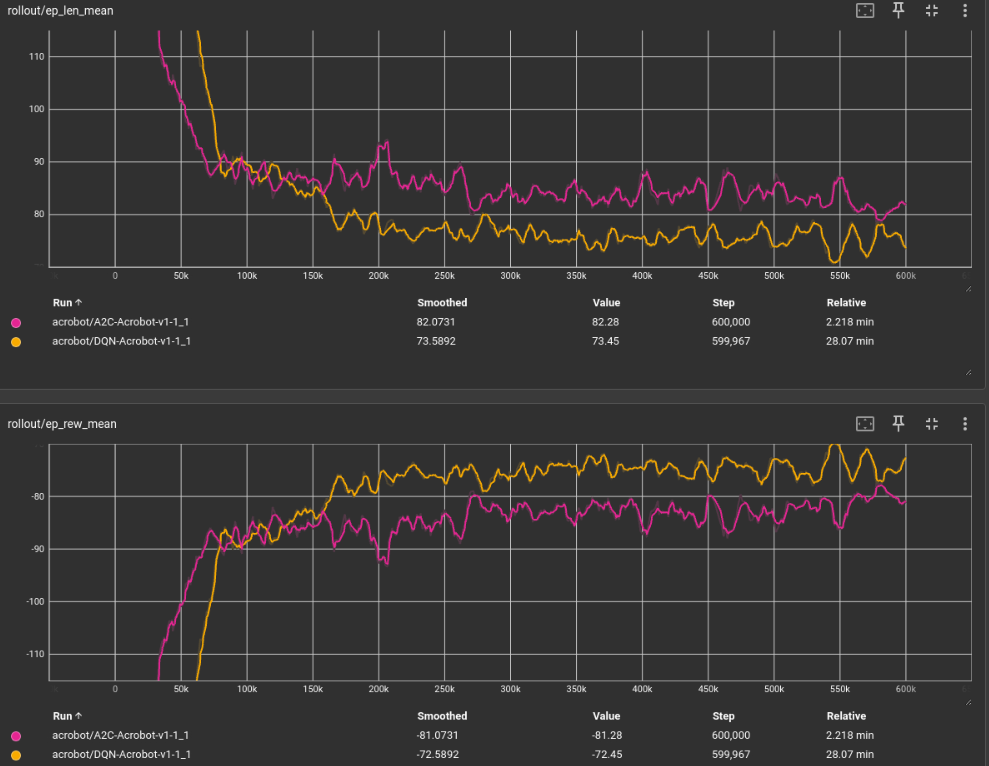
\includegraphics[width=7cm]{figs/Plataformas_Desarollo/TensorBoard.png}
  \end{center}
  \caption{Visualización de datos en TensorBoard.}
  \label{tensorboard}
\end{figure}

\section{Entornos de desarrollo}
\label{sec:des}

\subsection{Anaconda}
\label{sec:conda}

Anaconda\footnote{\url{https://www.anaconda.com/}} es una plataforma de distribución de software que facilita la gestión de entornos y librerías para el desarrollo de aplicaciones en Python. Permite crear entornos aislados con versiones específicas de Python y otras dependencias, lo que ayuda a evitar conflictos entre proyectos y a garantizar que las aplicaciones se ejecuten con las versiones requeridas de las bibliotecas. En este \ac{TFG}, se crea un entorno Anaconda que nos permita utilizar la versión 3.10 de Python, ya que es la que necesitaremos para utilizar EfficientVit.

\begin{code}[h]
\begin{lstlisting}[language=bash]

conda create -n tfg python=3.10
conda activate tfg

\end{lstlisting}
\caption[Creación del entorno Anaconda]{Creación y activación del entorno Anaconda.}
\label{cod:anaconda}
\end{code}

\subsection{Visual Studio Code}
\label{sec:vs_code}

Visual Studio Code\footnote{\url{https://code.visualstudio.com/}} es un editor de código gratuito y compatible con varias plataformas, diseñado para crear, modificar y depurar código en varios lenguajes de programación. Este software también incluye herramientas adicionales como extensiones que optimizan la escritura en diferentes lenguajes, autocompletado de código y terminales integrados para hacer más eficiente la ejecución y depuración.

\begin{figure}[ht]
  \begin{center}
    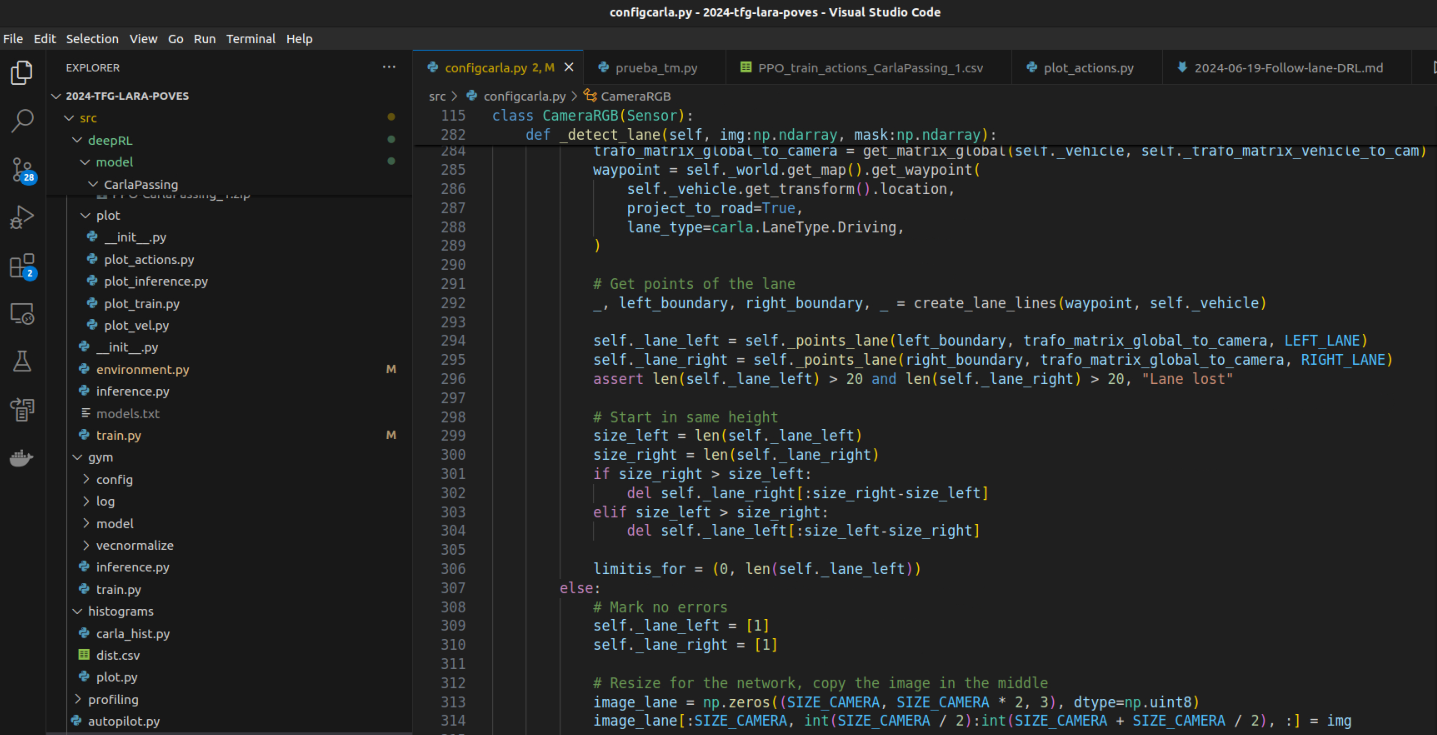
\includegraphics[width=10cm]{figs/Plataformas_Desarollo/visual_code.png}
  \end{center}
  \caption{Desarrollo en Visual Studio Code.}
  \label{foto_code}
\end{figure}

\newpage

En este \ac{TFG}, se utiliza Visual Studio Code como el editor principal para el desarrollo de todo el código, aprovechando sus extensiones para Python y YAML\footnote{\url{https https://www.ibm.com/es-es/topics/yaml}}, lo cual optimizó la productividad y facilitó la escritura del código.

\section{Herramientas para la detección de carril}
\label{sec:herramientas_carril}

Para la detección de carril, se ha utilizado la herramienta \textit{carla\_lane\_detector}, desarrollada por RoboticsLabURJC. Esta herramienta permite identificar con precisión las líneas que delimitan el carril dentro del simulador CARLA, proporcionando información crucial para el control y la navegación del vehículo autónomo, lo que permite además ajustar su trayectoria en función de la información obtenida. Existen dos técnicas principales para llevar a cabo esta detección: una basada en \ac{DL} y otra en información de CARLA.

\subsection{Detección \ac{DL}}
\label{sec:carril_dl3}

El modelo basado en \ac{DL} ha sido entrenado con imágenes tomadas del simulador CARLA y se ha implementado utilizando la librería PyTorch. Este modelo de segmentación está diseñado para identificar las líneas del carril en entornos simulados, aprendiendo patrones a partir de un conjunto amplio de datos y generando una máscara que indica la probabilidad de que cada píxel pertenezca a una de las líneas de carril. Sin embargo, este enfoque presenta algunas limitaciones, por ejemplo, si un vehículo está delante y oculta las líneas del carril, el modelo no es capaz de resolver esta situación, lo que podría llevar a una detección del carril imprecisa o incluso nula.

\begin{figure}[ht]
  \begin{center}
    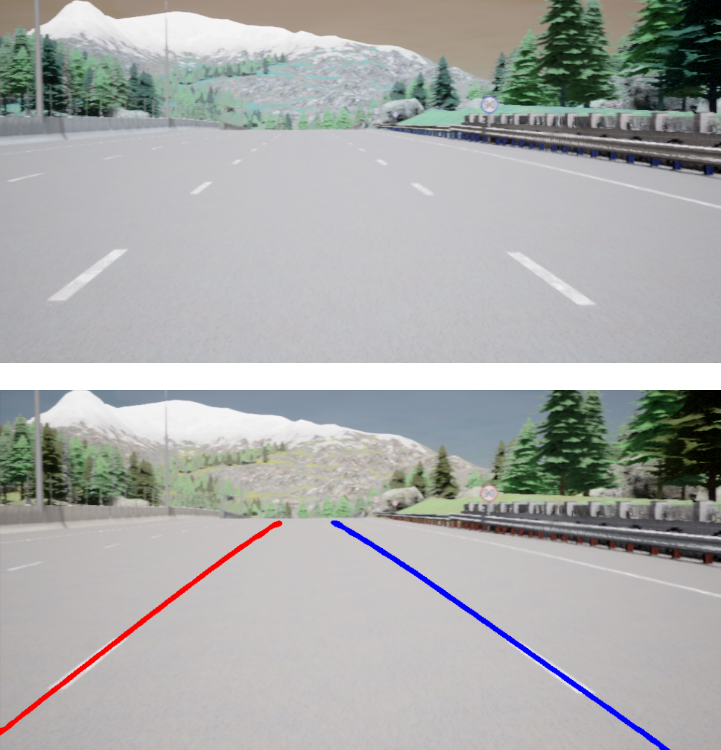
\includegraphics[width=13cm]{figs/Plataformas_Desarollo/carla_lane_dl.png}
  \end{center}
  \caption{Detección de carril basada en \ac{DL}.}
  \label{dl_lane}
\end{figure}

\subsection{Detección ground truth}
\label{sec:gt}

Por otro lado, la detección de carril basada en \textit{ground truth} aprovecha la ubicación del vehículo y la cámara dentro de CARLA para realizar la detección del carril. Gracias a la transformación de coordenadas entre el vehículo y la cámara, junto con la posición precisa del vehículo, es posible obtener los límites del carril en 3D, visión global en CARLA. Además, disponemos de la matriz intrínseca K, que permite la conversión de coordenadas de 2D a 3D. Utilizando esta matriz, los límites del carril pueden proyectarse a 2D. A diferencia de la solución basada en \ac{DL}, este enfoque no depende de la visibilidad directa de las líneas del carril, si hay elementos que obstruyen la visión, la detección sigue siendo precisa, ya que se basa en información global del entorno de CARLA y no en una imagen.

\begin{figure}[ht]
  \begin{center}
    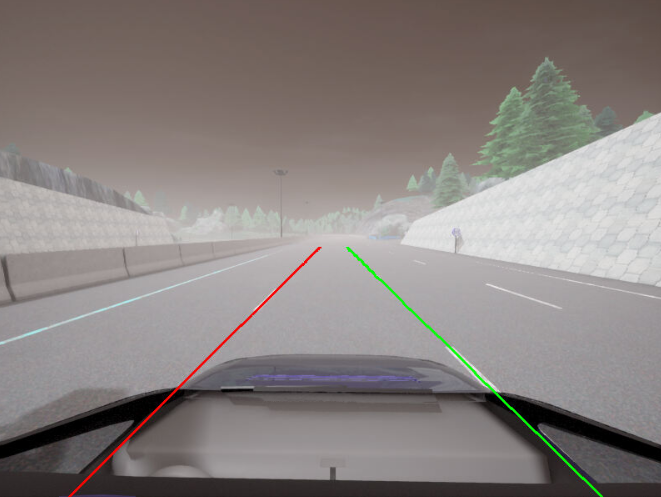
\includegraphics[width=7cm]{figs/Plataformas_Desarollo/ground_truth.png}
  \end{center}
  \caption{Detección de carril basada en \textit{ground truth}.}
  \label{dl_lane}
\end{figure}

\section{EfficientVit}
\label{sec:ef}

EfficientViT es un innovador módulo dentro de la familia de \textit{Vision Transformers}\footnote{\url{https://arxiv.org/pdf/1706.03762}}, utilizado con éxito en tareas como segmentación semántica, superresolución de imágenes y modelos de segmentación generalizados. Su principal ventaja es la significativa reducción de latencias sin perder rendimiento, haciendo posible su uso en aplicaciones de tiempo real. A diferencia de los modelos tradicionales que dependen de mecanismos de atención computacionalmente costosos o convoluciones de gran tamaño, EfficientViT emplea una atención lineal multiescala\footnote{\textbf{Multiescala:} enfoque que procesa información en distintos niveles de detalle simultáneamente para mejorar la eficiencia y precisión} ligera \cite{efficientvit}.

La segmentación es el proceso de dividir una imagen en regiones significativas para identificar objetos y se divide en dos tipos principales: segmentación semántica y segmentación de instancias. En la segmentación semántica, se asigna una clase a cada píxel de la imagen, pero no se distingue entre diferentes instancias de una misma clase. En cambio, la segmentación de instancias, no solo clasifica los píxeles en categorías, sino que también identifica y distingue las instancias individuales de un objeto. Por ejemplo, en una imagen con varios vehículos, la segmentación de instancias, además de clasificar los píxeles como vehículos, es capaz de diferenciar entre cada vehículo de forma individual.

En este \ac{TFG}, se utiliza el modelo EfficientViT Segmentation\footnote{\url{https://github.com/mit-han-lab/efficientvit/blob/master/applications/efficientvit_seg}} para detectar la calzada. Este modelo ha sido entrenado con \textit{Cityscapes Dataset}\footnote{\url{https://www.cityscapes-dataset.com/}}, diseñado para la comprensión semántica de escenas urbanas, centrándose en la segmentación de calles y objetos en entornos urbanos. Este \textit{dataset} incluye anotaciones poligonales, que marcan con precisión los objetos en las imágenes realizando una segmentación semántica densa, asignando una etiqueta a cada píxel de la imagen. Además, para objetos como vehículos y personas, se emplea segmentación de instancias.

\begin{figure}[ht]
\begin{center}
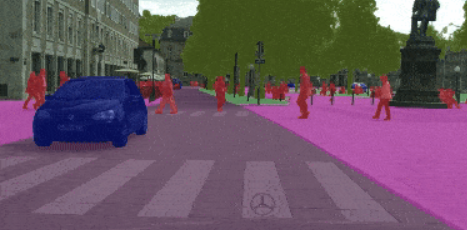
\includegraphics[width=7cm]{figs/Plataformas_Desarollo/resultado_ef.png}
\end{center}
\caption{Resultado de segmentación semántica con EfficientViT \cite{efficientvit-gif}.}
\label{foto_ef}
\end{figure}

Este conjunto de datos contiene imágenes reales tomadas en 50 ciudades durente diferentes estaciones del año, condiciones meteorológicas variadas y a distintas horas del día. Las imágenes fueron seleccionadas manualmente, asegurando una gran cantidad de objetos dinámicos, así como variación en el fondo y en la disposición de las escenas. \textit{Cityscapes Dataset} incluye un total de 5.000 imágenes con anotaciones detalladas y 20.000 con anotaciones más generales, cubriendo 30 clases de objetos urbanos. Esto lo convierte en un recurso muy útil para entrenar modelos de visión por computadora en entornos urbanos con muchos elementos.
\begin{figure}[ht]
\begin{center}
% Imagen con datos detallados del dataset
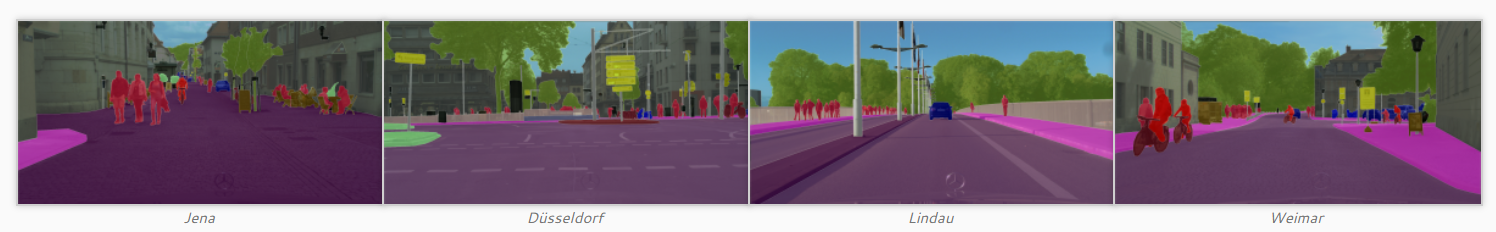
\includegraphics[width=15cm]{figs/Plataformas_Desarollo/detallado-ef.png}
\caption{Ejemplo de imagen con datos detallados de \textit{Cityscapes Dataset} \cite{cityscapes}.}
\label{foto_ef_detallado}
\vspace{0.5cm} % Espacio entre las dos imágenes
% Imagen con datos más generales del dataset
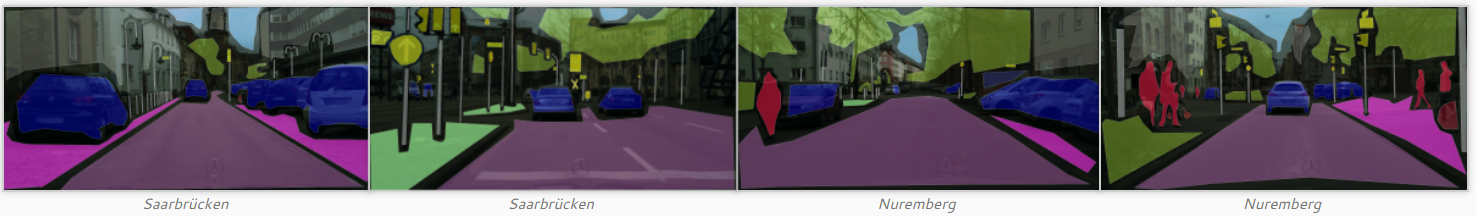
\includegraphics[width=15cm]{figs/Plataformas_Desarollo/no_detallado_ef.png}
\caption{Ejemplo de imagen con datos más generales de \textit{Cityscapes Dataset} \cite{cityscapes}.}
\label{foto_ef_general}
\end{center}
\end{figure}

\section{Entorno de simulación}
\label{sec:sim}
\subsection{CARLA}
\label{sec:carla}

CARLA\footnote{\url{https://github.com/carla-simulator/carla}} es un entorno de simulación de código abierto que se emplea en aplicaciones de conducción autónoma. CARLA se basa en \textit{Unreal Engine de Epic Games}\footnote{\url{https://www.unrealengine.com/en-US}}, lo que le permite generar entornos urbanos y rurales altamente detallados y realistas. Estos entornos son ideales para simular la interacción de los vehículos autónomos con el entorno, probando su capacidad de navegación, toma de decisiones y respuesta ante situaciones imprevistas.

\begin{code}[h]
\begin{lstlisting}[language=bash]

/opt/carla/CarlaUE4.sh -world-port=2000

\end{lstlisting}
\caption[Comando para lanzar el simulador CARLA]{Comando para lanzar el simulador CARLA.}
\label{cod:cmdcarla}
\end{code}

Este simulador destaca por su capacidad de recrear escenarios dinámicos con una amplia variedad de condiciones de tráfico, clima y paisajes urbanos, convirtiéndolo en una herramienta valiosa para la investigación en condiciones similares a las del mundo real. Para aprovechar estos entornos, utilizaremos \textit{scripts} de Python que nos permitirán personalizar las simulaciones, brindando flexibilidad para ajustar propiedades como el comportamiento de los vehículos o la configuración de los sensores.

\begin{figure}[ht]
\begin{center}
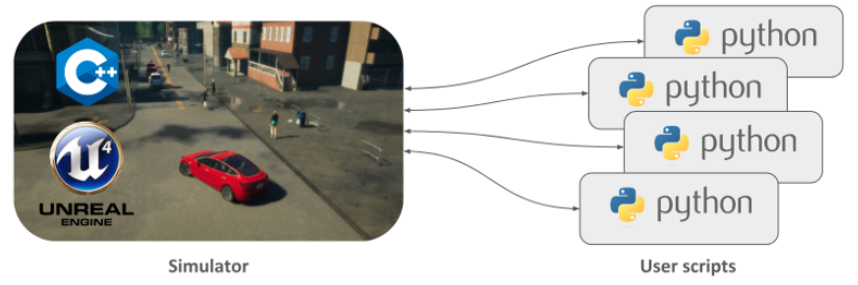
\includegraphics[width=9cm]{figs/Plataformas_Desarollo/carla.png}
\end{center}
\caption{Simulador CARLA.}
\label{carla}
\end{figure}

\newpage 

En CARLA, los mapas son modelos tridimensionales detallados de ciudades y sus infraestructuras viales, que no solo incluyen la geometría de las carreteras y edificios, sino también objetos interactivos como semáforos, señales de tráfico y otros elementos estáticos, los cuales pueden activarse o desactivarse según las necesidades del usuario. CARLA ofrece una amplia selección de mapas predefinidos que se pueden cargar directamente. Por otro lado, el mundo en CARLA se refiere al entorno completo de la simulación, que incluye el mapa, el clima, el tiempo, los vehículos, los peatones y otros elementos dinámicos, permitiendo crear una simulación realista y modificable en tiempo real para ajustar factores como la hora del día, las condiciones climáticas o el tráfico.

\subsubsection{Actores}

Los actores en CARLA son los elementos que realizan acciones dentro de la simulación y pueden interactuar con otros actores. Existen varios tipos de actores, cada uno con funcionalidades específicas:

\begin{itemize}
\item \textit{Sensores.} Los sensores\footnote{\url{https://carla.readthedocs.io/en/latest/core_sensors/}} son actores capaces de producir un flujo de datos y existen diversos tipos disponible. La mayoría de los sensores se anexan a un vehículo para recopilar información sobre su entorno, indicando la localización y rotación respecto al mismo. Los sensores escuchan datos y, cuando reciben información, llaman a una función descrita mediante una expresión \textit{Lambda}\footnote{\url{https://docs.python.org/3/reference/expressions.html}}. 

	\begin{code}[h]
	\begin{lstlisting}[language=python]
	
	camera_bp = blueprint_library.find('sensor.camera.rgb')
	camera = world.spawn_actor(camera_bp, transform, attach_to=vehicle)
	camera.listen(lambda image: image.save_to_disk('output/%06d.png' % image.frame))

	\end{lstlisting}
	\caption[Configuración de cámara RGB en CARLA]{Configuración de cámara RGB en CARLA.}
	\label{cod:camara_carla}
	\end{code}


\item \textit{Espectador.} El espectador proporciona un punto de vista dentro de la simulación. Puede utilizarse para mover la vista en la ventana del simulador.
\item \textit{Señales de tráfico y semáforos.} En CARLA, solo las señales de \textit{stop}, ceda el paso y los semáforos son considerados actores.

\item \textit{Vehículos.} Los vehículos en CARLA son un tipo especial de actor que simula la física de los vehículos de ruedas real. Utilizan un controlador que define los atributos físicos del vehículo y otro que gestiona los comandos de conducción: aceleración, dirección y freno. CARLA ofrece varios tipos de vehículos (coches, motocicletas y camiones...\footnote{\url{https://carla.readthedocs.io/en/latest/catalogue_vehicles/}}), además de una gran variedad de modelos. El vehículo que se desea controlar, al que se le añaden los sensores, conocido como \textit{Ego Vehicle}, será el agente en el proceso de aprendizaje. Si indicamos esta condición al simulador, este renderiza solo la zona cercana a este vehículo para optimizar recursos.

	\begin{code}[h]
	\begin{lstlisting}[language=python]
	
	vehicle_vp = world.get_blueprint_library().find(vehicle_type)
	vehicle_vp.set_attribute('role_name', 'hero') # Ego vehicle
	ego_vehicle = world.spawn_actor(vehicle_bp, transform)
	ego_vehicle.apply_control(carla.VehicleControl(throttle=0.5, steer=0.1, brake=0.01))

	\end{lstlisting}
	\caption[Configuración de \textit{Ego Vehicle} en CARLA]{Configuración de \textit{Ego Vehicle} en CARLA.}
	\label{cod:ego_carla}
	\end{code}
    \item \textit{Peatones.} Los peatones funcionan de manera similar a los vehículos. El control sobre ellos se proporciona mediante controladores.
\end{itemize}

En este \ac{TFG} se utiliza como \textit{Ego Vehicle} el modelo \textit{Lincoln MKZ 2020}\footnote{\url{https://carla.readthedocs.io/en/latest/catalogue_vehicles/\#lincoln-mkz-2020}}, sobre el cual solo se controlarán los actuadores de giro y aceleración. El acelerador (\textit{throttle}) tiene un rango de 0 a 1, mientras que el giro (\textit{steer}) varía entre -1 y 1, donde -1 es giro a la izquierda y 1 a la derecha. Para simular el tráfico, se emplea un camión\footnote{\url{https://carla.readthedocs.io/en/latest/catalogue_vehicles/\#carla-motors-carlacola}} controlado por el autopiloto de CARLA, ya que, al no contar con cristales en la parte trasera, facilita la detección mediante el \ac{LiDAR}.

Al vehículo principal se le añaden tres tipos de sensores:

\begin{itemize}
\item \textit{Detector de colisión}\footnote{\url{https://carla.readthedocs.io/en/latest/ref_sensors/\#collision-detector}}. Este sensor registra un evento cada vez que el vehículo colisiona con un objeto en el entorno. Para identificar contra qué vehículo se ha chocado, se debe consultar el atributo \textit{other\_actor} en los datos del sensor.

\item \textit{Cámara RGB}\footnote{\url{https://carla.readthedocs.io/en/latest/ref_sensors/\#rgb-camera}}. La cámara RGB actúa como una cámara convencional, capturando imágenes de la escena. Se pueden configurar distintos parámetros, como las dimensiones de la imagen y el campo de visión. En este caso, se establecen dimensiones de 512 × 512 píxeles para garantizar compatibilidad con EfficientVit. Para consultar la matriz que define la imagen, debemos mirar en los datos de salida el atributo \textit{raw\_data}.

\item \textit{Sensor \ac{LiDAR}}\footnote{\url{https://carla.readthedocs.io/en/latest/ref_sensors/\#lidar}}. Este sensor simula un \ac{LiDAR} rotativo mediante \textit{ray-casting}, generando puntos al agregar un \ac{LiDAR} por cada canal distribuido en el campo visual vertical. Los datos se codifican en cuatro dimensiones: las primeras tres corresponden a la posición en \textit{x, y, z}, y la cuarta representa la intensidad de la señal reflejada. Se pueden configurar parámetros como los ángulos del campo de visión superior, inferior y horizontal, siendo en nuestro caso un láser de 360º, mientras que el resto de los atributos se mantienen con los valores por defecto. Además, es posible ajustar la frecuencia de rotación y la cantidad de puntos por segundo, lo cual adaptaremos dependiendo de los \ac{FPS} alcanzados. Al igual que en la cámara, los datos de salida incluyen la nube de puntos completa en el atributo \textit{raw\_data}.
\end{itemize}

\subsubsection{Traffic Manager}

El \ac{TM} es el módulo encargado de controlar los vehículos en modo piloto automático dentro de una simulación. Su propósito principal es recrear condiciones de tráfico urbano realistas en el entorno simulado. Los usuarios tienen la posibilidad de personalizar ciertos comportamientos para configurar escenarios específicos de aprendizaje, para simular diferentes circunstancias de conducción.

El \ac{TM} está integrado en el lado cliente de CARLA, y es necesario especificar el puerto de conexión para su funcionamiento. Los usuarios pueden ajustar parámetros del flujo de tráfico, permitiendo, forzando o incentivando comportamientos específicos. Por ejemplo, se puede configurar que los vehículos ignoren los límites de velocidad, cambien de carril de forma obligatoria o adopten comportamientos personalizados. Estas capacidades permiten experimentar y simular situaciones para el entrenamiento y evaluación de sistemas de conducción autónoma.

En nuestro caso, los entrenamientos estarán limitados al uso del autopiloto para el coche delantero con una velocidad fija e ignorando completamente las señales de tráfico para realizar el control adaptativo el tráfico y el adelantamiento. 

\begin{code}[h]
	\begin{lstlisting}[language=python]
	
	tm = client.get_trafficmanager(port)
	vehicle.set_autopilot(True, tm.get_port())  
	tm.ignore_lights_percentage(vehicle, 100) 
	self._tm.set_desired_speed(vehicle, velocity) #km/h
\end{lstlisting}
\caption[Configuración del \textit{Traffic Manager} en CARLA]{Configuración del \textit{Traffic Manager} en CARLA.}
\label{cod:tm_carla}
\end{code}

\section{Hardware}
\label{sec:hw}
\subsection{Servidor Thor}
\label{sec:thor}

CARLA es un simulador que requiere una gran capacidad computacional. La ejecución de algoritmos de aprendizaje por refuerzo, combinados con diversas redes neuronales para la percepción, incrementa aún más esta demanda de potencia. Para satisfacer estos requisitos, es fundamental disponer de los recursos de hardware adecuados. Lo ideal es contar con una o varias \ac{GPU}, ya que están optimizadas para el procesamiento paralelo masivo, lo que en nuestro caso aceleraría significativamente tanto la simulación como el entrenamiento de modelos de \ac{IA}. 

El servidor Thor, ubicado en la Escuela de Ingeniería Superior de Fuenlabrada de la \ac{URJC}, forma parte de la granja de servidores con \ac{GPU} de RoboticsLabURJC. Este servidor está diseñado para tareas que requieren un alto rendimiento, ya que su arquitectura \textit{x86\_64} y el potente procesador \textit{AMD Ryzen Threadripper 7960X} lo hacen adecuado para aplicaciones exigentes. La velocidad del procesador varía dependiendo de la carga de trabajo, oscilando entre 545 MHz en reposo y hasta 7786 MHz cuando se necesita el máximo rendimiento, lo que contribuye tanto a la optimización del consumo energético como a la mejora del desempeño del sistema. En cuanto al almacenamiento, el servidor cuenta con 125 GiB de memoria \ac{RAM} y su capacidad total de disco es de 24,8 TB, distribuida entre las diferentes unidades de almacenamiento.

Además, el servidor está equipado con una \ac{GPU} NVIDIA GeForce RTX 4090 con 24 GB de memoria, lo que permite no solo gestionar cargas computacionales intensivas, sino también facilitar el entrenamiento y la inferencia de modelos en tiempo real. Esta capacidad es crucial para el desarrollo y las pruebas de este \ac{TFG}, como se puede observar en la Figura \ref{fig:thor_nvidia}.

\begin{figure}[ht]
  \centering
  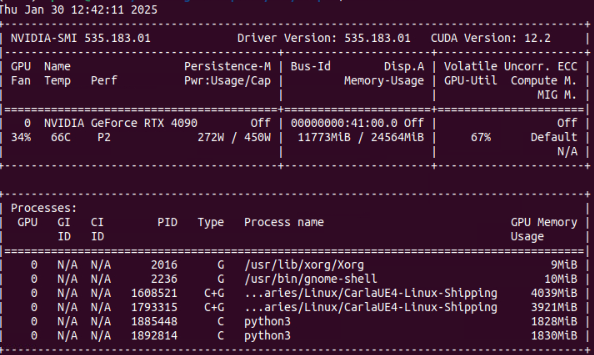
\includegraphics[width=9cm]{figs/Plataformas_Desarollo/thor.png}
  \caption{Servidor Thor equipado con una \ac{GPU}.}
  \label{fig:thor_nvidia}
\end{figure}










\input{capitulos/Diseño}
%\chapter{Conclusiones}
\label{cap:capitulo5}

En este TFG se han cumplido los objetivos marcados durante su desarrollo. Primero la creación de algoritmos de
navegación autónoma para drones para resolver la problemática de seguimiento de carril en entornos de carreteras. 
En segundo lugar la utilización de algoritmos basados en Inteligencia Artificial y aprendizaje no supervisado
con el fin de evaluar su efectividad. Tercero, analizar el desarrollo de aplicaciones de navegación autónoma drones
utilizando el simulador foto-realista Airsim junto con el middleware robóticos ROS empleando una arquitectura de
comunicación cliente-servidor. 

En conclusión, se comenta los objetivos que se han cumplido a lo largo del desarrollo como los requisitos cumplidos
que se expusieron en el capítulo 2, englobando líneas futuras dentro del trabajo. 

\section{Objetivos cumplidos}
\label{objetivos_cumplidos}

Los objetivos presentados en la sección \ref{sec:descripcion}, han sido cumplidos exitosamente 
\begin{enumerate}
    \item Se logró la instalación y configuración del simulador Airsim junto con ROS, estableciendo la comunicación efectiva
    entre dos equipos mediante protocolos de red. 
    \item Se implementó satisfactoriamente un sistema perceptivo capaz de realizar una detección del carril utilizando 
    redes neuronales junto con algoritmos de aprendizaje automático.
    \item Se implementó satisfactoriamente un sistema de control utilizando técnicas de aprendizaje por refuerzo, en especial Q-learning 
    para lograr el seguimiento del carril del dron de manera robusta y eficaz.
    \item Se completó de manera exitosa la aplicación para el seguimiento del carril para drones, haciendo uso del sistema perceptivo y de control
    \item Se han completado análisis efectivos para tanto para el sistema perceptivo como los comportamientos de control de PID y Q-learning, demostrando que el comportamiento
    de Q-learning es capaz de generalizar mejor en comparación con el controlador PID.
\end{enumerate}

\section{Requisitos satisfechos}
\label{requisitos_satisfechos}

En la sección \ref{sec:requisitos} se presentaron los requisitos que ha tenido este TFG, que se han ido resolviendo 
de la siguiente forma: 

\begin{enumerate}
    \item Durante todo el proceso del trabajo se utiliza Airsim junto con Unreal Engine como entorno de simulador.
    \item Los comportamientos desarrollados durante el trabajo se ha utilizado la estructura de ROS junto con la comunicación
    del entorno de simulación Airsim. 
    \item La navegación autónoma basada en aprendizaje por refuerzo ha demostrado ser lo suficiente robusta y eficiente en los
    diferentes trayectos dentro del escenario Coastline. 
    \item El comportamiento Q-learning junto con el sistema perceptivo han demostrado ser reactivos y poder reaccionar al entorno en tiempo real
    durante la navegación del dron.
    \item Uso del algoritmo de Q-Learning para desarrollar el comportamiento sigue-carril basados en aprendizaje por 
    refuerzo.
\end{enumerate}


\section{Balance global y competencias adquiridas}
\label{balance_global_competencias_adquiridas}
Durante el desarrollo de este TFG, el desafío de implementar una aplicación de navegación autónoma de drones basada en
aprendizaje por refuerzo y uso de redes neuronales resultó ser un proceso complejo y enriquecedor. Además de que la
combinación de aprendizaje por refuerzo e Inteligencia Artificial es una estrategia viable y efectiva para la
navegación autónoma de drones. Los resultados obtenidos son prometedores y sugieren que, con más investigación y
desarrollo, estos sistemas pueden ofrecer soluciones robustas y eficientes para la navegación autónoma en una variedad
de entornos sumando la arquitectura de conexión que se llego a implementar para ello. 

Al comienzo de este trabajo apenas tenía suficientes conocimientos básicos sobre Inteligencia Artificial enfocada en
redes neuronales y aprendizaje por refuerzo. Destacando que ha sido mi primer trabajo de investigación en donde he
aprendido múltiples conceptos, así como adquirir técnicas de análisis de errores que han ido apareciendo durante todo
el proceso. Destacando las siguientes competencias: 

\begin{itemize}
    \item Organización en cuanto a tiempos y tareas utilizando la metodología Kanban.
    \item Nuevos conocimientos en la utilización de simuladores robóticos.
    \item Nuevos conocimientos dentro del área de Inteligencia Artificial, así como redes neuronales y algoritmos de
    aprendizaje no supervisado. 
    \item Nuevos conocimientos desde cero sobre comportamientos basados en aprendizaje por refuerzo.
    \item Capacidad de analizar diferentes resultados recogidos en los diferentes comportamientos implementados.
    \item Mejora en la capacidad de implementar una arquitectura distribuida entre ambos equipos.
    \item Nuevos conocimientos sobre la integración de ROS junto con aplicaciones externas.
    \item Capacidad de documentación a la hora de desarrollar los diferentes comportamientos. 
\end{itemize}

\section{Líneas futuras}
\label{lineas_futuras}
Hemos obtenido resultados exitosos y satisfactorios a lo largo del TFG, dentro del campo de la navegación autónoma de drones, no obstante, existen diferentes líneas futuras que se
podrían desarrollar a partir de este trabajo.

\begin{itemize}
\item Re-entrenar la red YOLOP con un nuevo dataset teniendo en cuenta la posición y el ángulo de la cámara abordo del dron en diferentes entornos de Airsim.
\item Búsqueda de algoritmos alternativos que produzcan mejores resultados a la hora de refinar resultados de redes neuronales de segmentación.
\item Búsqueda sobre la infraestructura que existe entre el simulador PX4 Autopilot y Airsim, para tener mejores
comportamientos en cuanto a rendimiento y latencia.
\item Mejorar los sistemas de seguimiento de carril de aprendizaje por refuerzo sin las propias limitaciones que puede
presentar el algoritmo de Q-learning, usando algoritmos de Deep Reinforcement Learning.
\item Probar el comportamiento en diferentes escenarios distintos, con circuitos con curvas más cerradas, con situaciones de tiempo
adversas. 
\end{itemize}
%\begin{appendices}
\chapter{Anexo}  % Se numera como "6. Anexo"
\label{cap:anexo}

A continuación, se muestran las referencias a las Figuras usadas en este \ac{TFG}. Las imágenes no incluidas en este capítulo han sido obtenidas durante el desarrollo del proyecto.\newline

\begin{tabular}{ | m{4cm} | m{10cm}| m{1cm} | }
    \hline
    \textbf{Referencia de las imágenes} & \textbf{Enlaces de donde se ha obtenido}  \\
    \hline
    \ref{fig:aut-levels} & \url{https://www.autobild.es/practicos/coche-autonomo-seis-niveles-conduccion-cuales-son-como-funcionan-cuando-llegaran-490005} \\ 
	\hline
	\ref{fig:leganes-photo} & \url{https://www.leganes.org/web/guest/w/leganes-pionero-en-la-puesta-en-marcha-de-un-proyecto-de-autobus-urbano-sin-conductor} \\
	\hline
	\ref{fig:coche-geddes} & \url{https://www.20minutos.es/noticia/1591770/0/norman-bel-geddes/diseno/futuramar} \\
	\hline
	\ref{fig:vamp} & \url{https://www.politico.eu/article/delf-driving-car-born-1986-ernst-dickmanns-mercedes/} \\
	\hline
	\ref{fig:waymo} & \url{https://www.appventurez.com/blog/ai-in-self-driving-cars/} \\
	\hline
	\ref{fig:tesla} & \url{https://www.tesla.com/original-modely} \\
	\hline
	\ref{fig:cruise} & \url{https://www.youtube.com/watch?v=uCGkAIdOVjw&t} \\
	\hline
	\ref{fig:baidu} & \url{https://www.enter.co/chips-bits/gadgets/tomaria-un-taxi-conducido-por-un-robot-de-noche-esta-ciudad-tiene-el-servicio/} \\
	\hline
	\ref{fig:cir3} & \url{https://carla.readthedocs.io/en/latest/map_town03/} \\
	\hline
	\ref{fig:mapa} & \url{https://carla.readthedocs.io/en/latest/map_town04/} \\
	\hline
	\ref{fig:comma} & \url{https://comma.ai/shop/comma-3x} \\
	\hline
	\ref{fig:accidentes} & \url{https://www.craftlawfirm.com/autonomous-vehicle-accidents-2019-2024-crash-data/} \\
	\hline
	\ref{fig:ml} & \url{https://telefonicatech.com/blog/semi-supervised-learningel-gran-desconocido} \\
\end{tabular}

\begin{tabular}{ | m{4cm} | m{10cm}| m{1cm} | }
	\ref{fig:yolo} & \url{https://www.330ohms.com/es-es/blogs/blog/deteccion-de-objetos-con-yolo} \\
	\hline
	\ref{fig:rl} & \url{https://www.researchgate.net/figure/Figura-1-Esquema-del-aprendizaje-por-re-fuerzo_fig1_365016137} \\
	\hline
	\ref{fig:aws} & \url{https://ai4sme.aisingapore.org/2020/05/train-a-viable-model-in-45-minutes-for-aws-deepracer-beginner-challenge-virtual-community-race-2020/} \\
		\hline
	\ref{fig:foto_ef} & \url{https://github.com/mit-han-lab/efficientvit/blob/master/assets/cityscapes_l1.gif/} \\
	\hline
	\ref{fig:foto_ef_detallado} \ref{fig:foto_ef_general} & \url{https://www.cityscapes-dataset.com/examples/} \\
	\hline
	\ref{fig:carla} & \url{https://carla.readthedocs.io/en/0.9.7/getting_started/} \\
	\hline
\end{tabular}

\end{appendices}





%\begin{appendices}
    \chapter*{Anexo II}
    \addcontentsline{toc}{chapter}{Anexo II}
    \label{cap:anexoII}
\setcounter{page}{1}
Durante las primeras fases del desarrollo del TFG, se desarrolló un teleoperador\footnote{\url{https://github.com/RoboticsLabURJC/2022-tfg-barbara-villalba/tree/main/src/teleop_drone}} 
para analizar el comportamiento del dron frente a los comandos de posición y velocidades lineales y angulares.
Para la implementación del mismo, se utilizó el simulador Gazebo junto con PX4 Autopilot, Mavros y ROS. 

En primer lugar, se llevó a cabo la configuración del dron, específicamente el modelo Iris, dentro del archivo de configuraciones del propio launcher de PX4. Una vez cargado 
el modelo en Gazebo, se procedió a realizar la tarea de teleoperación. Para el desarrollo de la aplicación de teleoperación, se desarrollaron 
dos nodos diferentes: la interfaz, en la cual se visualiza la imagen de la cámara abordo del dron junto con sliders y botones para comandar velocidades lineales y angulares, despegue y aterrizaje, y
el teleoperador, donde se procesan los datos que se reciben a través de la interfaz. 

El nodo de la interfaz, esta construida a partir de la biblioteca PyQt5, donde se captura la imagen del dron calculando sus frames por segundo junto con la creación diferentes botones y sliders para comandar 
la orden que se quiere seguir. Entre los botones, se implementan las funciones de despegue (Take Off) y aterrizaje (Land), junto con los modos de control: posición y velocidad.
. Respecto a los sliders, se tiene en total
4: control de posición en el eje x, control de posición en el eje z, control de velocidad lineal en el eje x e control de velocidad angular en el eje z.  Con este nodo se envían las ordenes que 
posteriormente serán procesadas en el nodo de la teleoperación.

En el nodo de teleoperación, se gestionan las peticiones realizadas desde la interfaz mediante la subscripción a través de topics. Con dichos topics, se puede determinar qué comando
se desea enviar al dron. Para el control tanto de posición como de velocidad, junto con los comandos Take off y Land, se utilizan PX4 y Mavros. En la figura \ref{fig:Teleoperador}, 
se muestra el simulador Gazebo junto con el dron Iris y el nodo de la interfaz para comandar el comportamiento deseado del dron. Esta aplicación de teleoperación es una buena herramienta 
para el control del movimiento que se puede tener en un dron.

\begin{figure}[H]
    \centering
    \begin{minipage}{1.0\textwidth}
      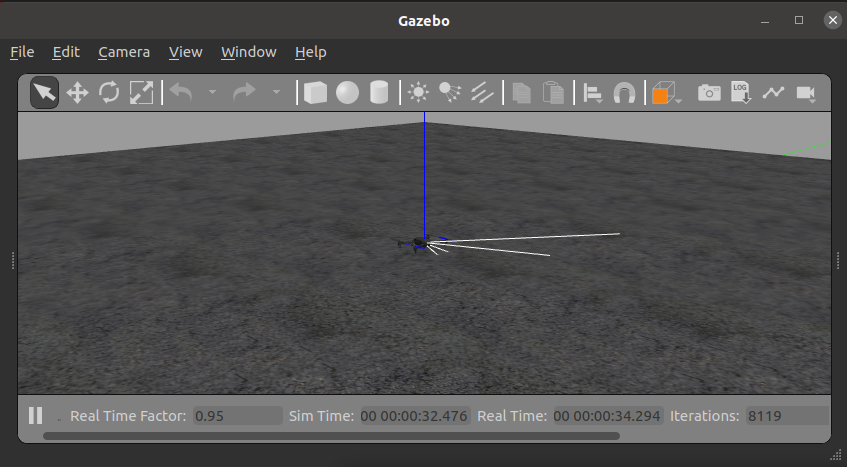
\includegraphics[width=\linewidth]{figs/anexo/gazebo.png}
    \end{minipage}
    \begin{minipage}{1.0\textwidth}
      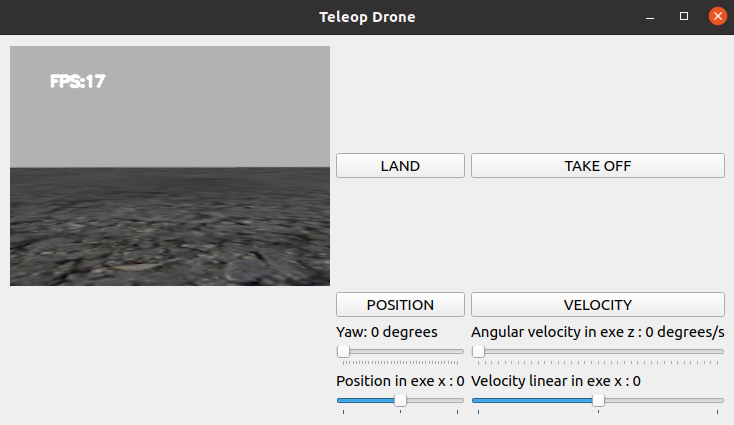
\includegraphics[width=\linewidth]{figs/anexo/interfaz.png}
    \end{minipage}
    \caption{Teleoperador}
    \label{fig:Teleoperador}
    \vspace{-1.5em}
  \end{figure}

\end{appendices}









\clearpage
\thispagestyle{empty}

\printindex \nocite{*}
\appendix
\bibliographystyle{apalike} \bibliography{bibliografia}

\end{document}
